\chapter{Kernel CN:\ Static semantics}%

\margintoc{}%
%
I have covered a large amount of background to the type system so far:
\intro{Core}, liquid types, bidirectional type systems, linear types, precise
separation logic assertions, monadic syntax for the latter and its relation to
kernel syntax for types, let-normalisation and explicit resource terms in
\kl{ResCore}. I use all of these ingredients in defining the type system for
\kl{kernel CN} that I will explain in this chapter. Some of the sections will
based on my contributions to~\sidetextcite[4.5cm]{pulte2023cn}%

The \kl{Kernel CN} type system is ordinary \kl{CN}, defined over \kl{ResCore}
instead of \kl{Core}, without any type or resource inference. In particular, It
requires that that all universal quantifiers are explicitly instantiated, that
all existential quantifiers have explicit witnesses, and all resource
operations are embedded into the program itself as linearly typed proof terms.
It does not require proof terms for the logical properties, since by
construction all of the entailments fall into the decidable SMT fragment; many
rules rely on this. The lack of inference make it a simpler language for which
to prove type soundness, whilst still demonstrating all the key ingredients
mentioned above. Since it handles the majority of C, the entire system is very
large, and so I will only discuss the main features.

There are some additional minor differences between the implementation and the
formalisation. As I mentioned \nameref{sec:desugaring}, the formalisation has a
richer grammar of resources: this makes defining predicates to represent tagged
unions more succinct, and allows for opening predicates in more cases. The
formalisation assumes that iterated resources output arguments have type array
of records, whereas the implementation uses records of arrays.\sidenote{This
purely a notational convenience so I could avoid inventing syntax for indexing
over an arbitrary record of arrays.}

Along with the type system, I briefly discuss a formalisation of two different
elaboration algorithms: one for inferring instantiations of logical quantifiers,
one for inferring indices for \kl{iterated} predicates. Because of a change
to the inference scheme used by \kl{CN}, the latter algorithm is no longer
used.\sidenote{\href{https://github.com/rems-project/cerberus/commit/7c2c0a364a4373e4eb109f32d01cc9584f51e81f}{Commit
7c2c0a36.}}\label{sn:new-inf-statics}

\section{Contexts}

The contexts for the static semantics consist of four parts: (1) $\mathcal{C}$
containing the computational variables from the Core program; (2) $\mathcal{L}$
containing purely logical variables mentioned in specifications; (3) $\Phi$,
the constraint context, containing a list of (non-quantified) SMT constraints;
and (4) $\mathcal{R}$ a \emph{linear} context containing the resources
available at that point during type-checking. I assume a constraint context of
only non-quantified constraints because users are required to manually
instantiate quantified constraints to use them.

\section{Pure values and expressions}

\kl{ResCore} programs have both computational and logical (ghost) terms.
Every such term, computational or ghost, has a \kl{base type} $\beta$,
which are things like unit, booleans, (mathematical) integers,\sidenote{After the formalisation was completed,
\kl{CN} switched from using mathematical unbounded integers to bit vectors
(\href{https://github.com/rems-project/cerberus/commit/8fdd4198750446de3b44d00f9e8f185db9610fab}{around
commit 8fdd41987}) to better support common bit-twiddling idioms, used heavily
in the buddy allocator in pKVM, without resorting to lots of lemmas about
uninterpreted functions.} locations, and records and user-defined algebraic datatypes of
other base types. Each C type $\tau$ is mapped to a corresponding base type $\beta_\tau$
\textemdash{} for example, $\beta_{\mathtt{int*}} = \mathsf{loc}$.

Logical terms are variously referred to as ${term}$, ${iguard}$ (for boolean
index guards of iterated predicates), ${ptr}$ (for pointers), ${init}$ (for
initialisation status), ${value}$ (for pointees), ${iarg}$ (for input mode
arguments to predicates),  ${oarg}$ (for output arguments for type record or
array of records), and later, ${alloc}$ (for constraints about the allocation
history).

As seen in \cref{fig:typing-pval-pexpr}, the rules for pure
values\sidenote{Because \kl{Core} factors out the memory object model, it also
factors out the precise representation of memory objects such as integers,
pointers, arrays and structs, so I have followed a similar factorising in
the structure of the typing judgements, and left the representation of these
values abstract.} are very simple pure value synthesis judgements of the form
$\mathcal{C} \vdash \mathit{pval} \Rightarrow \colorbox{red!8}{\beta}$;
given computational context and a pure value, synthesise a base type.

Building on the rules for pure values, the pure expression synthesis judgements
are not that much more complicated either: $\mathcal{C}; \mathcal{L}; \Phi
\vdash \mathit{pexpr} \Rightarrow \outpol{pure\_ret}$. Given a computational
context, a logical context, a constraint context and a pure expression,
synthesise a \emph{pure} return type (a return type without any resources or
logical variables). The use of return types starts to introduce a few more of
the refinement type features gestured at earlier. The type $\Sigma y {:}
\beta.\ \phi(y) \wedge{} I$ is simply the usual refinement type $\{ \, y \in
\beta \mid\phi(y) \, \}$, translated over to the grammar of types in \kl{Kernel
CN}. Recall that $\Sigma$ is used to bind a computational value in a
\emph{return} type, so these types are simply expressing, symbolically, in
constraints, that these expressions will evaluate to a value. Pure values are
simply lifted into the grammar of SMT constraints with an equality constraint;
pure expressions are lifted similarly but with their equivalent symbolic
computation.

\begin{figure*}[tp]
    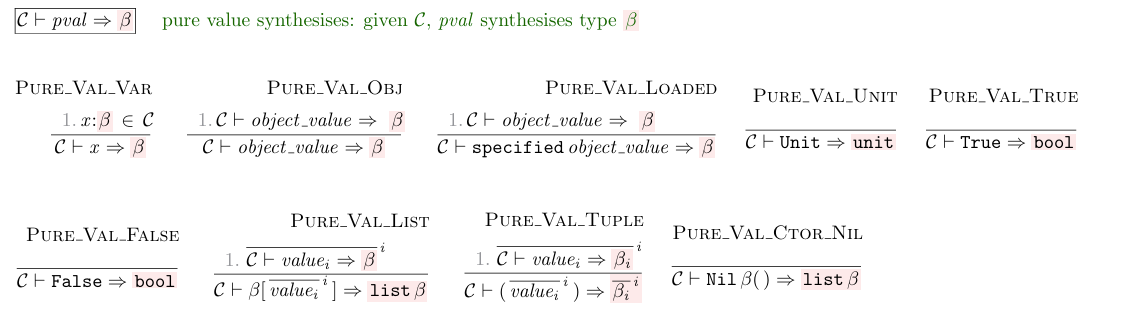
\includegraphics{figures/kernel-pval-typing}
    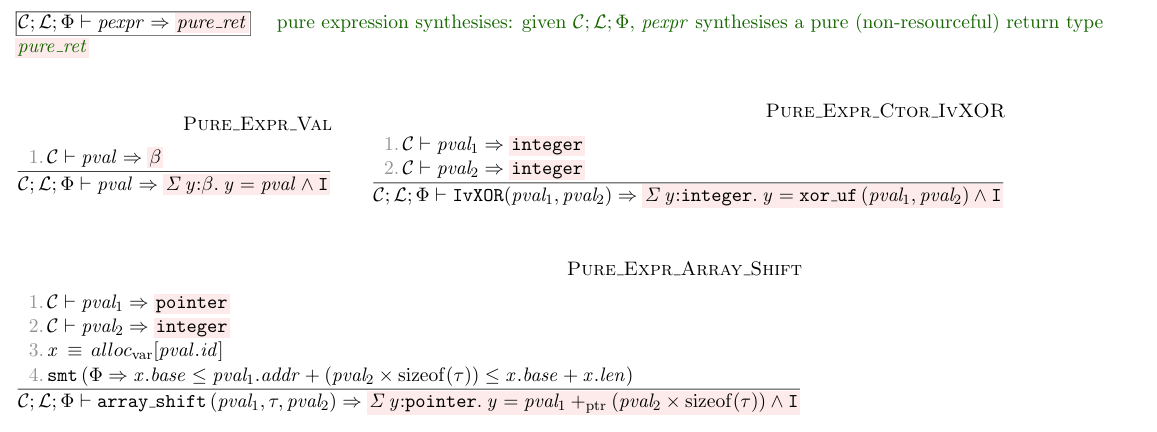
\includegraphics{figures/kernel-pexpr-typing}
    \caption{Selection of \kl{Kernel CN} typing rules for pure values and
        expressions.}\label{fig:typing-pval-pexpr}
\end{figure*}

\section{Top-level pure value values and expressions}

Whilst the rules for typing \emph{top-level} pure values and pure expressions
share the same context as typing pure values and expressions, they differ in
that they are \emph{checking} judgements instead of synthesising ones, of the
form $\mathcal{C}; \mathcal{L}; \Phi \vdash \mathit{tpexpr} \Leftarrow
\mathit{pure\_ret}$ (and similarly for $\mathit{tpexpr}$). Given the
computational, logical and constraint contexts, check the top-level value (or
expression) has satisfies this type.

Here we start to see the let-normalisation (\cref{sec:rescore}) and the
bidirectional (\cref{sec:bidir-subtyping}) approaches pay off. A top-level pure
value (i.e.\ the result of evaluating a pure expression) is checked against a
pure return type by checking if the constraint attached to it is true given the
context by calling the SMT solver, which is another reason why the constraints
being decidable is important and helpful. Similarly, the constructs we would
like to avoid (\coreinline{undef()} and \coreinline{error()}) check against % chktex 36
\emph{any} type, so long as the constraint context is inconsistent (can prove
$\mathsf{false}$). Top-level if-expressions synthesise a type for their condition,
but then check the branches, with an extra constraint on the true or false
value of the condition. Similarly, top-level let-expressions synthesise a type
for the bound expressions, and a constraint on the \emph{shape} bound value to
the context, and then check the body of the let.

The constraint on the shape of the bound value is produced by a judgement which
given a computational pattern (one inherited from Core) and a base type, it
produces a computational context and a term corresponding to the \emph{shape}
of the value according to the pattern match. For the sake of simplicity, I
assume all patterns are complete.

\begin{figure*}[tp]
    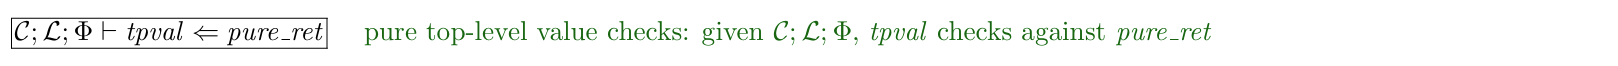
\includegraphics{figures/kernel-tpval-typing}
    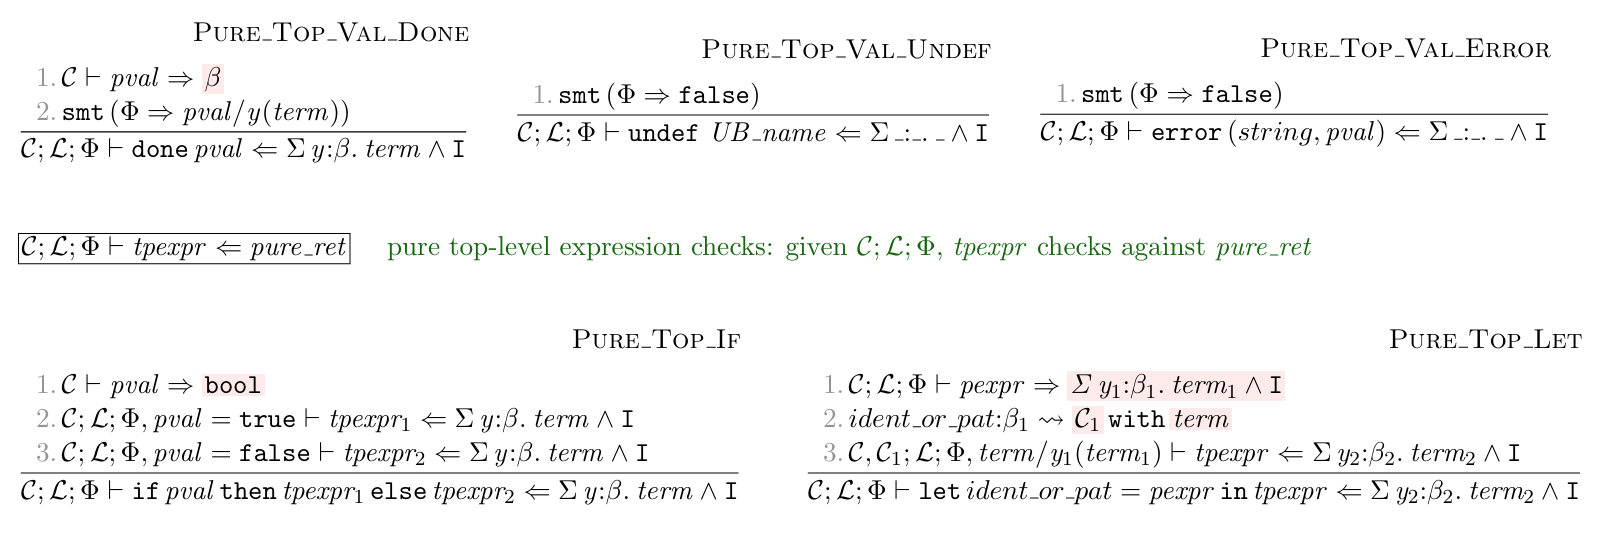
\includegraphics{figures/kernel-tpexpr-typing}
    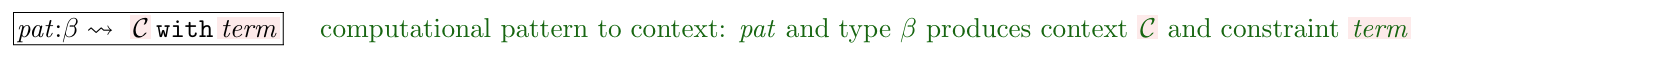
\includegraphics{figures/kernel-pat-comp-typing-1}
    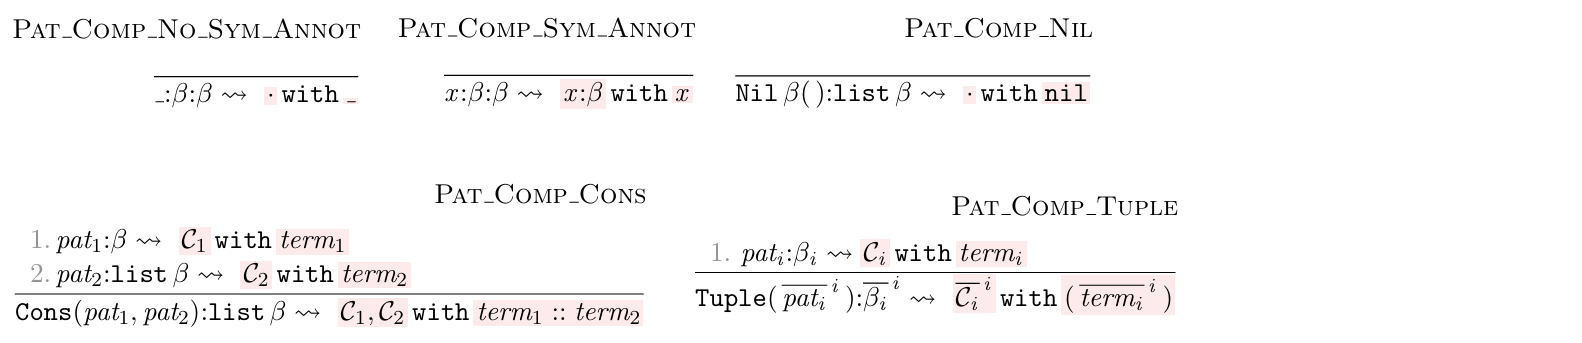
\includegraphics{figures/kernel-pat-comp-typing-2}
    \caption{Selection of \kl{Kernel CN} typing rules for top-level pure values and
        expressions, including the translation of computational patterns into a
        computational context used in the \coreinline{let} rule.}\label{fig:typing-tpval-tpexpr}
\end{figure*}

\section{Resource terms}\label{sec:typing-res-terms}

\begin{figure*}[tp]
    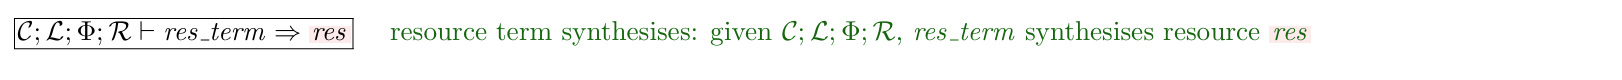
\includegraphics{figures/kernel-res-term-synth-1}
    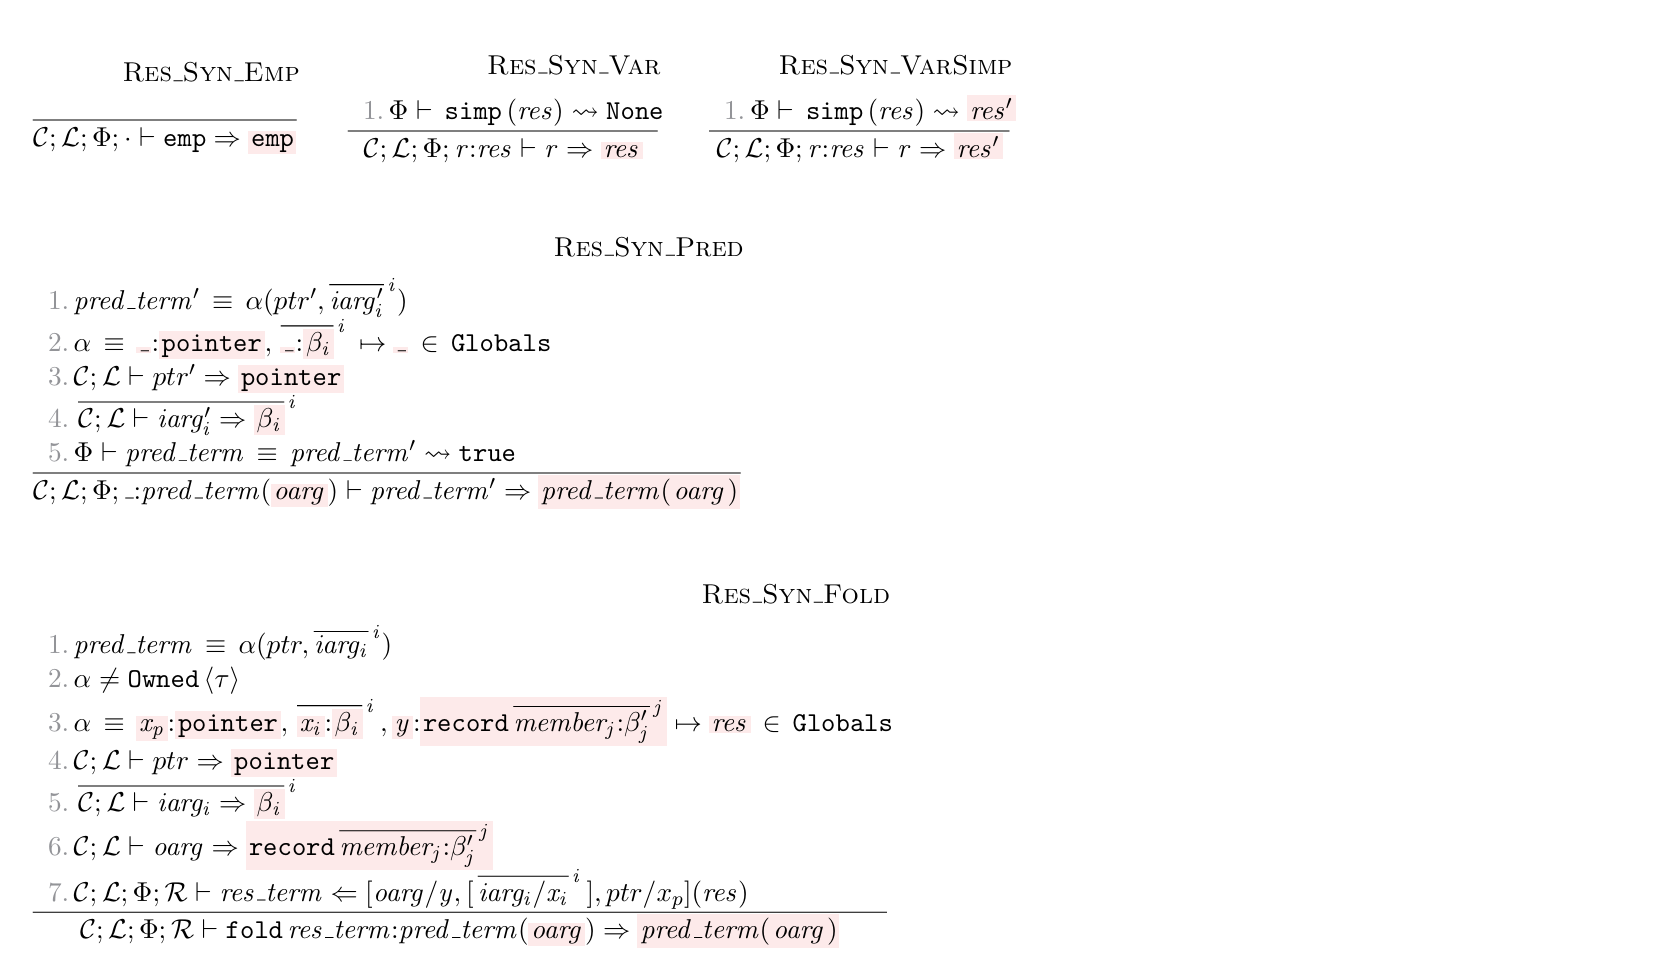
\includegraphics{figures/kernel-res-term-synth-2}
    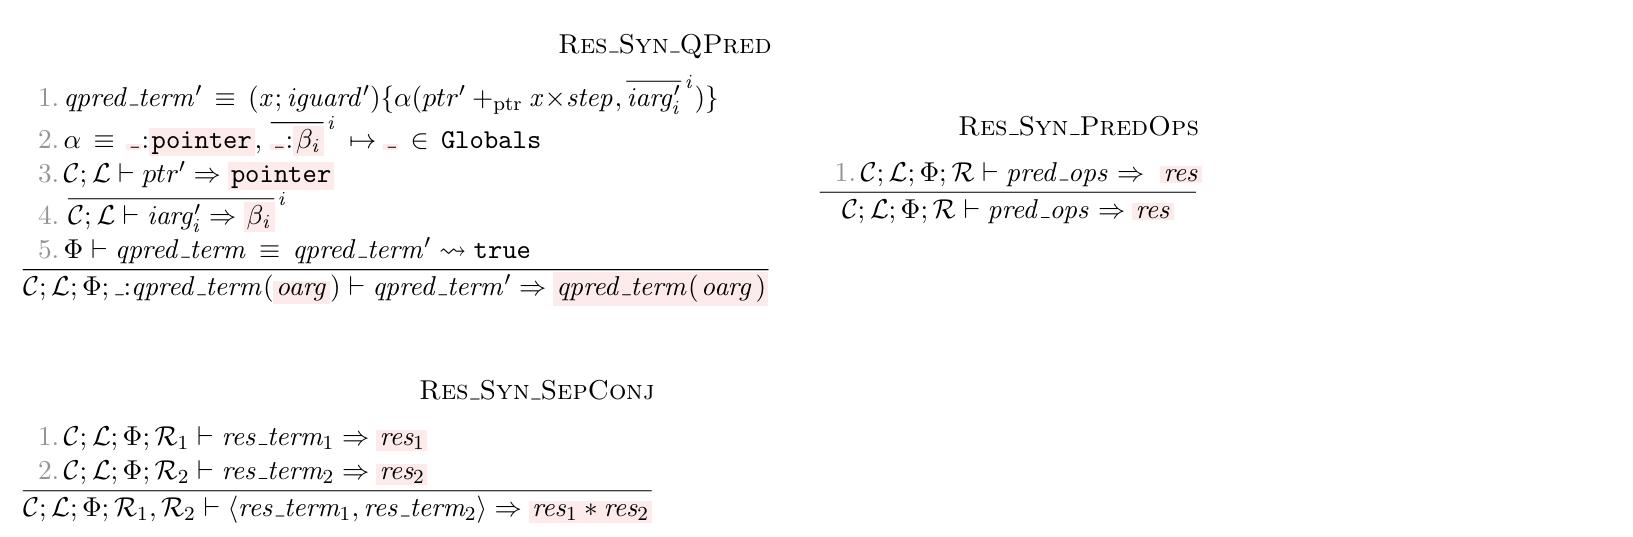
\includegraphics{figures/kernel-res-term-synth-3}
    \caption{Selection of \kl{Kernel CN} synthesising typing rules for resource
        terms.}\label{fig:typing-res-term-synth}
\end{figure*}

Typing resource terms requires the addition of an extra \emph{linear} context
$\mathcal{R}$ of resources. I will start with the synthesising judgements first,
and move on to checking judgements after.

\subsection{Synthesis for resource terms}\label{subsec:synth-res-term}

As visible in \cref{fig:typing-res-term-synth}, unsurprisingly, $\mathsf{emp}$
requires an empty context, and a variable use requires a singleton context.
Using variables also \emph{simplifies} them; simplification here just means
stripping as many top-level \coreinline{if}s off when their conditions are
provable to be true or provable to be false. Predicate (iterated and otherwise)
terms synthesise their types by checking the arguments (input and output) are
of the correct type. Note that (a) because of linearity, the context is a
singleton and (b) the lookup into the context is by predicate name $\alpha$ and
its input arguments, not by variable and (c) the output argument is synthesised
from the context. For ownership predicates, the input is the location, but the
output will be the initialisation status and the value stored at that location:
the program terms are not required to know what is in the heap.

Only user-defined predicates can be folded, so $\mathsf{Owned}\langle\_\rangle$
is excluded.\sidenote{Needs to be updated for $\mathsf{Alloc}$ too.} A term to
be folded is simply the (partially-evaluated) body of some predicate, so it
does not have the information required to know which predicate it could belong
to, especially because resources can and are moved between predicate. Hence,
morally, $\mathsf{fold}$ should be checked, not synthesised. However, in a
prior version of \kl{CN}, users were required to manually fold and unfold
predicates, and (by accident) that annotation was placed in an
indeterminately-sequenced expression, which also includes things like memory
actions. Memory actions are not well suited to be checked and are best
synthesised, and so this forced the fold/unfold annotations, and the resource
terms it contained, to also be synthesising.\sidenote{Of course, despite all
this, because the resource assertions are all assumed to be precise, we
could infer the output argument, but {Kernel CN} is meant to assume no
inference of instantiations to logical quantifiers, i.e.\ output arguments of
resources.} Hence, $\mathsf{fold}$ terms are annotated with the predicate which
they are meant to be folded into, so that the $\mathit{res\_term}$ it carries
can be \emph{checked} against the \emph{definition} (`body') of that predicate,
with the input and output arguments substituted in (after the arguments
are checked to be of the correct type).

\subsection{Synthesis for predicate operations}

Predicate operations are also synthesising and have their own judgement. And
because these operations can combine more than one kind of resource, they need
to synthesise separating conjunctions, so the rule for them is also
synthesising.

For space, I only present the rules for turning ownership of fixed size array
into an iterated separating conjunction and back (\cref{fig:typing-predops}).

The first rule says that if $\mathit{res\_term}$ synthesises ownership of a
fixed size array, then the iteration of that synthesises an iterated separating
conjunction for ownership over the indices of that array ($0$ to
$n-1$).\sidenote{The notational hacks in this rule are a bit too cute and
difficult to explain, should probably change them.} The second rule does the
inverse, but includes some additional checks to prevent two adjacent locations
of the same type but belonging to different allocations, being indexable from
a single base pointer.

\begin{figure*}[tp]
    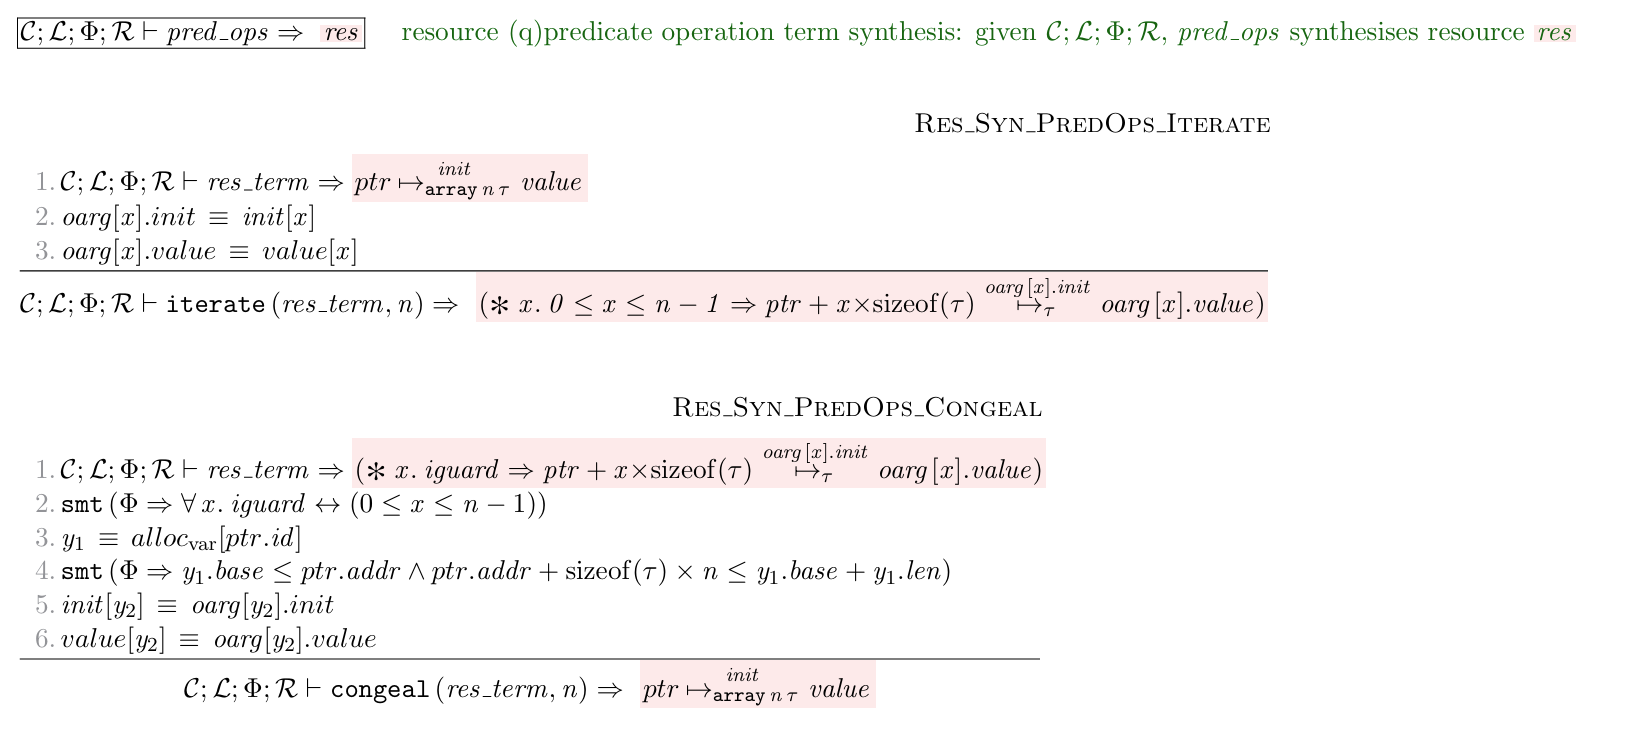
\includegraphics{figures/kernel-predops-typing}
    \caption{Selection of \kl{Kernel CN} synthesising typing rules for
        predicate operations.}\label{fig:typing-predops}
\end{figure*}

\subsection{Checking for resource terms}\label{subsec:checking-res-terms}

Lastly for the resource terms, we come to the checking rules. Resource terms
which represent constraints do not carry the constraint in them, and so need a
checking rule to learn them and prove them with a call to the SMT solver.
Similarly, because it is impossible to infer existential types in the general
case,\sidenote{Consider a heap $1 \mapsto 1$, and consider that all of $\exists
x.\ 1 \mapsto 1$, $\exists x.\ x \mapsto 1$, $\exists x.\ 1 \mapsto x$
(imprecise), $\exists x.\ x \mapsto x$ are valid inferences for it.} this too
is checking, and is straightforward since the instantiation is part of the
term, so it can be substituted into the type, which in turn can check the
$\mathit{res\_term}$ it carries.

As I mentioned earlier (\cref{subsec:res-terms}), \emph{any} resource term can
introduce an ordered-disjunction, and so any resource term can be checked by
it. Furthermore, at most \emph{one} of the branches may be checked, and which
one depends on whether the condition or its negation can be proven. In the
situation that neither is possible, I call the condition (and the resource)
\intro{under-determined} (with respect to a constraint context). In this case,
the system may attempt to synthesise a type for the term and check that the
synthesised type is equal to the ordered-disjunction. Only variables can
synthesise an ordered-disjunction type, that too only if the condition is
under-determined (otherwise simplification will reduce it to either branch).
Separating conjunctions are also checked to allow for the case where an
existential or an ordered-disjunction are in the sub-components.

\begin{figure*}[tp]
    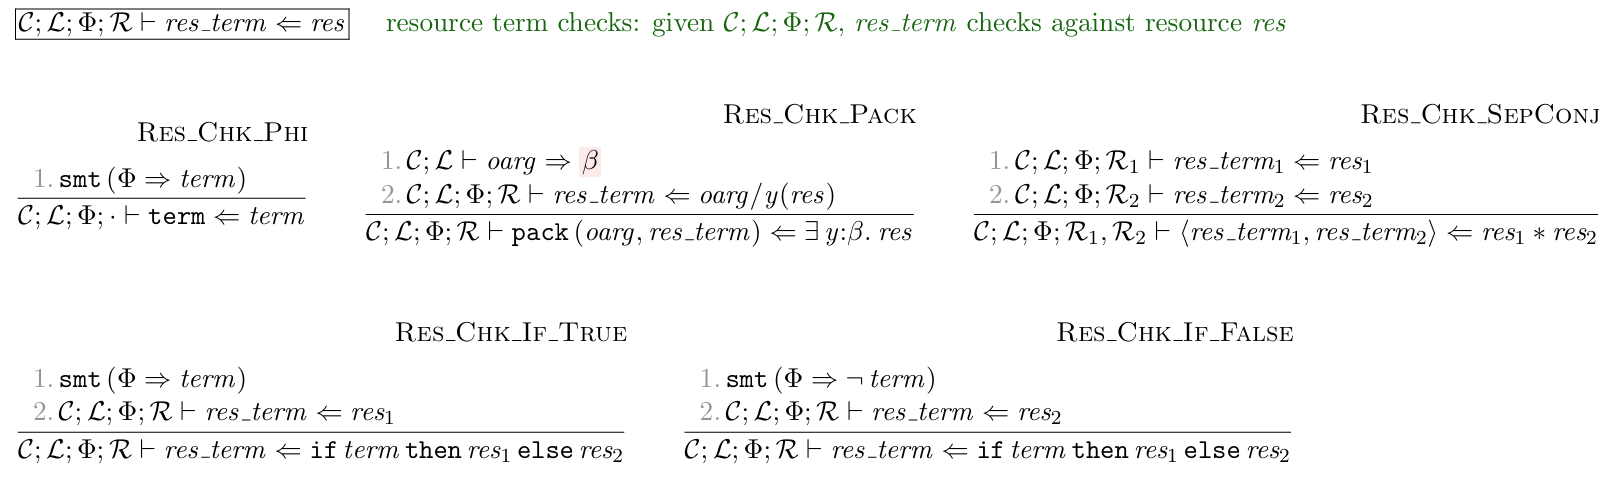
\includegraphics{figures/kernel-res-term-check}
    \caption{Selection of \kl{Kernel CN} checking typing rules for
        resource terms.}\label{fig:typing-res-term-check}
\end{figure*}

At any point, if the term cannot be checked by any other rule, the system can
switch to synthesising a type and then comparing whether the two types are
structurally equal, modulo SMT provability (\cref{fig:typing-res-term-check}).

\begin{marginfigure}
    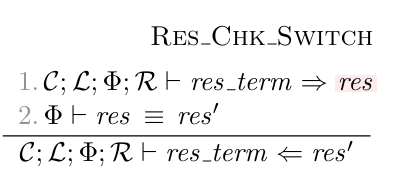
\includegraphics{figures/kernel-res-term-switch}
    \caption{Switching from checking to synthesising types for resource
        terms.}\label{fig:typing-res-term-switch}
\end{marginfigure}

\section{Memory actions and pointer operations}

As with resource terms, memory actions require all the contexts (computational,
logical, constraint and resource). The judgement $\mathcal{C} ; \mathcal{L} ;
\Phi ; \mathcal{R} \vdash \mathrm{mem\_action} \Rightarrow
\outpol{\mathrm{ret}}$ means that given the contexts and a memory action,
it synthesises a return type.

The rule for \coreinline{create()} is a bit busy because of % chktex 36
constraints on allocations required by the C standard (in premise 2), which I
will ignore. For now, the main thing to note is that the return type speaks of
the pointer to the newly created allocation as a computational value $y_p$,
constraints on pointer $y_p$ as required by the C standard, a unconstrained
logical (ghost) value for the pointee of the new allocation $x$, and the
finally the two resources it creates. The first is ownership of an
uninitialised piece of memory, at address $y_p$, and the second is an
allocation token $\mathsf{Alloc()}$ which is related to the memory object model
in \nameref{sec:cn-vip}.

In contrast, the rules for loads, stores and kill are quite simple. Loads
consume ownership of an initialised piece of memory\sidenote{For further
flexibility, loads of structs and unions could can be partially or completely
uninitialised, as allowed by the C standard, see
note~\ref{sn:partial-init-read}.}, check if the address of the load and the
address of the resource are symbolically equal, and synthesise a return type
mentioning the loaded value and ownership of the loaded location. Stores are
similar, but with extra checks on the stored value, which is also mentioned in
the ownership that is synthesised in the return type. Lastly, the rule for
\coreinline{kill()} is the converse of the one for \coreinline{create()}, % chktex 36
in that it \emph{consumes} the ownership and allocation token for a location
and synthesises a return type with no resources.\sidenote{I need to add the
rule for dynamic allocations.}

\begin{figure*}[tp]
    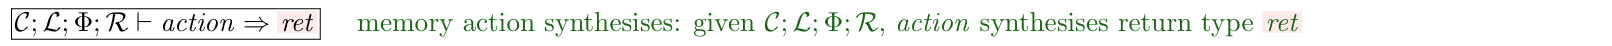
\includegraphics{figures/kernel-mem-action-typing-1}
    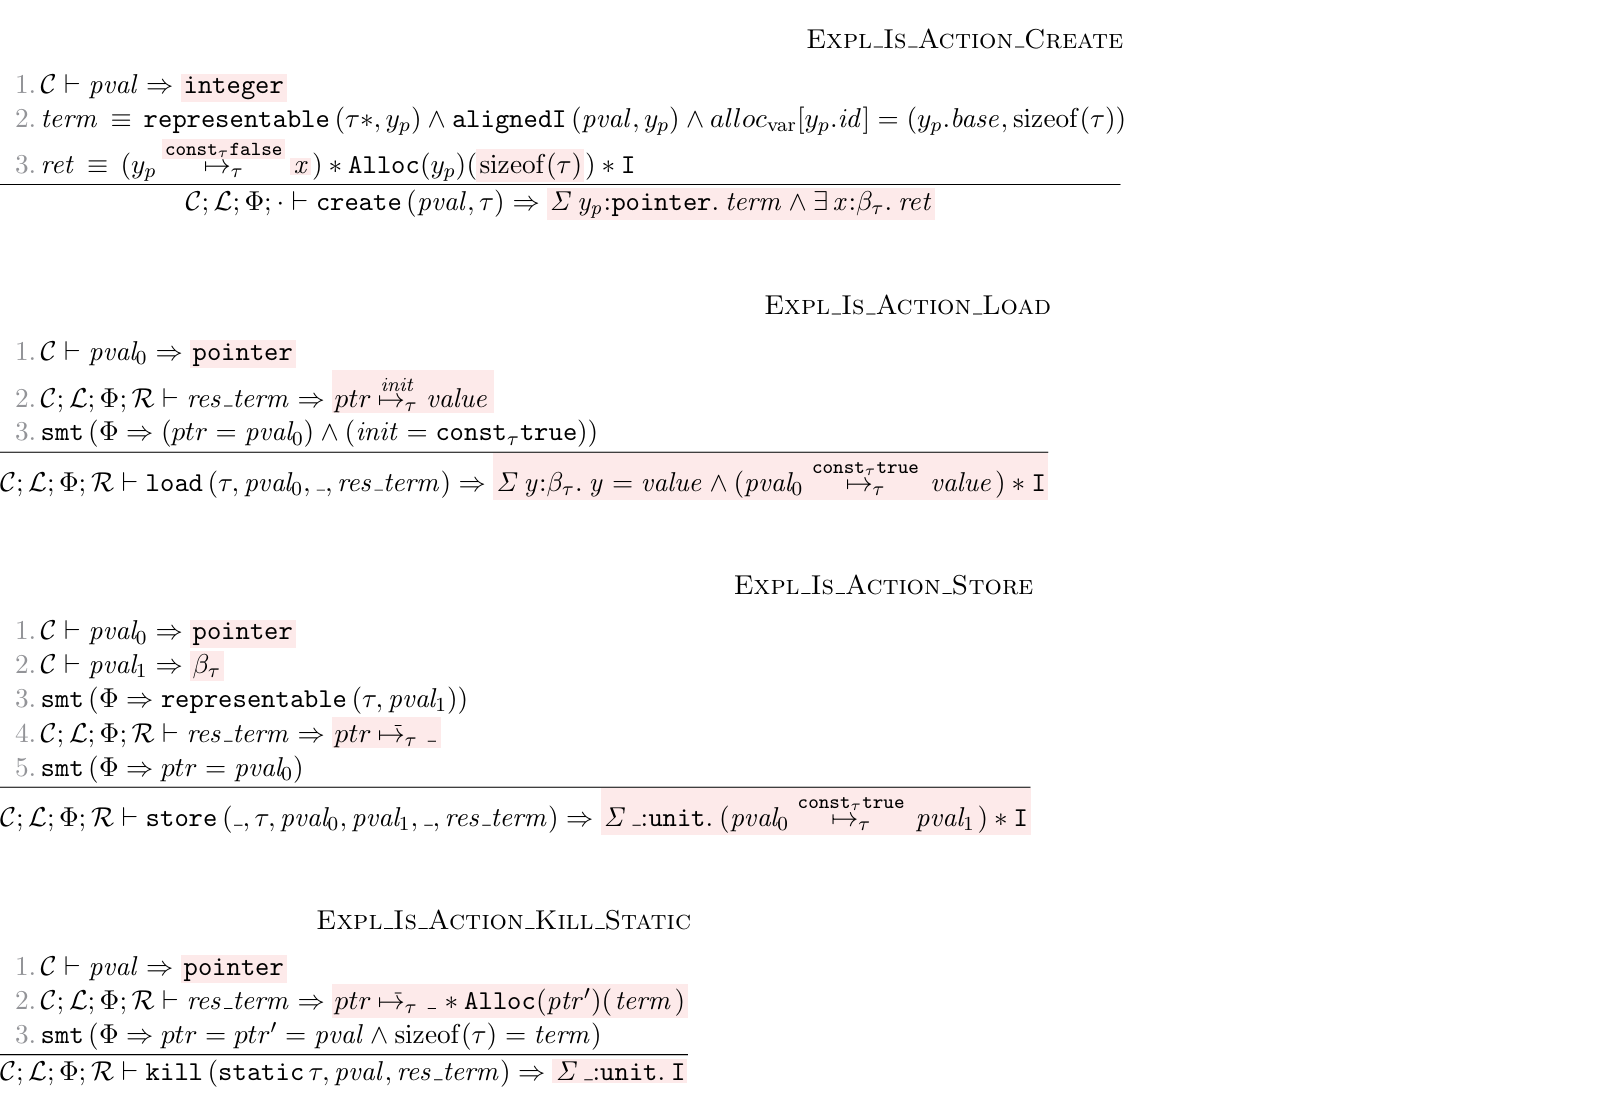
\includegraphics{figures/kernel-mem-action-typing-2}
    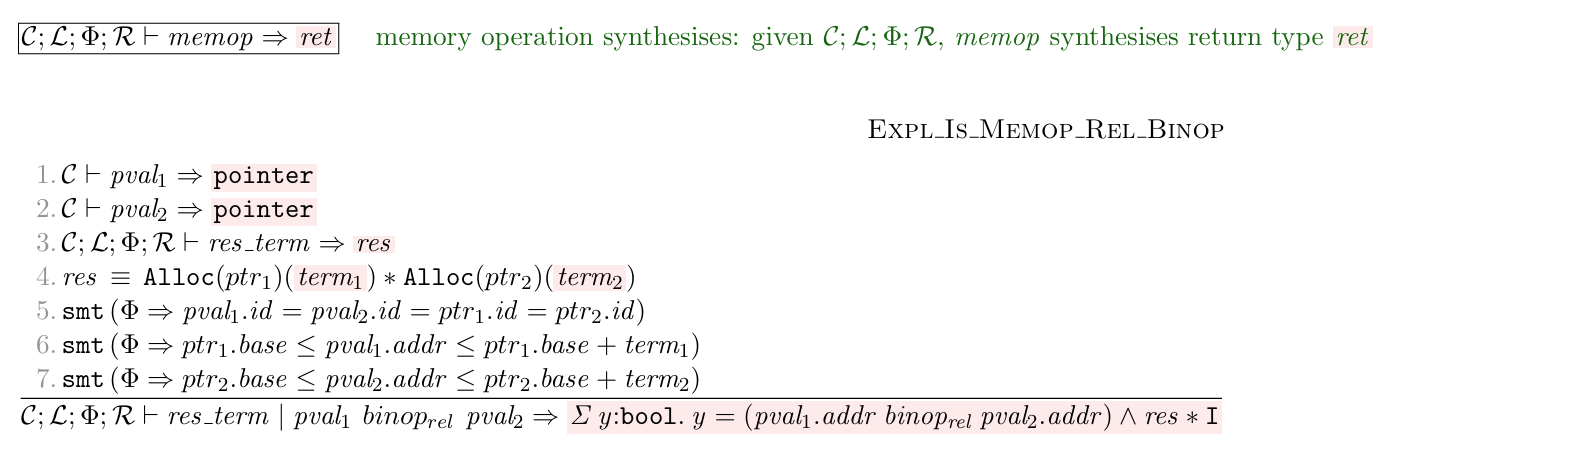
\includegraphics{figures/kernel-memop-typing}
    \caption{\kl{Kernel CN} typing rules for memory actions, and a select rule
        for typing a memory operation.}\label{fig:typing-mem-action}
\end{figure*}

Rules for typing memory operations, i.e.\ `effectful' pointer operations which
require not only for the pointer to be live, but satisfy certain allocation
bounds checks, also synthesise a return type. There are many of them, but they
share the same principles so it suffices to only explain one
(\cref{fig:typing-mem-action}).\sidenote{Update the rule to adjust the pointer
liveness check and notationally simplify the bounds checks into one line.}
Using a binary relational operator (not equality) is only valid if both
pointers are live, belong to the same allocation and have addresses which are
in that allocation's bounds. These constraints are all checked by the SMT
sovler, and the return type synthesises the result of that relational operator
applied to the addresses of those pointers, plus any resources consumed to
prove the pointer is live.

\section{Spine judgement}

There are two parts of the grammar which use spine, lists of values. The first
is its typical use in calls to pure Core functions, elaborated C functions, and
effectful Core procedures, as well as to the \coreinline{run()} % chktex 36
operator. Second is the less typical one, in \emph{top-level return values},
usually marked with \coreinline{done()}. So far, I have been showing % chktex 36
how expressions have return types, and so this is how to type the values to
which those expressions step.

Either way, the process for checking them is the same, and so the simplicity
gained by desugaring the \kl{CN} types into kernel types
(\cref{sec:desugaring}) pays off in the straightforward specification of these
rules (\cref{fig:typing-spine}).

\begin{figure*}[tp]
    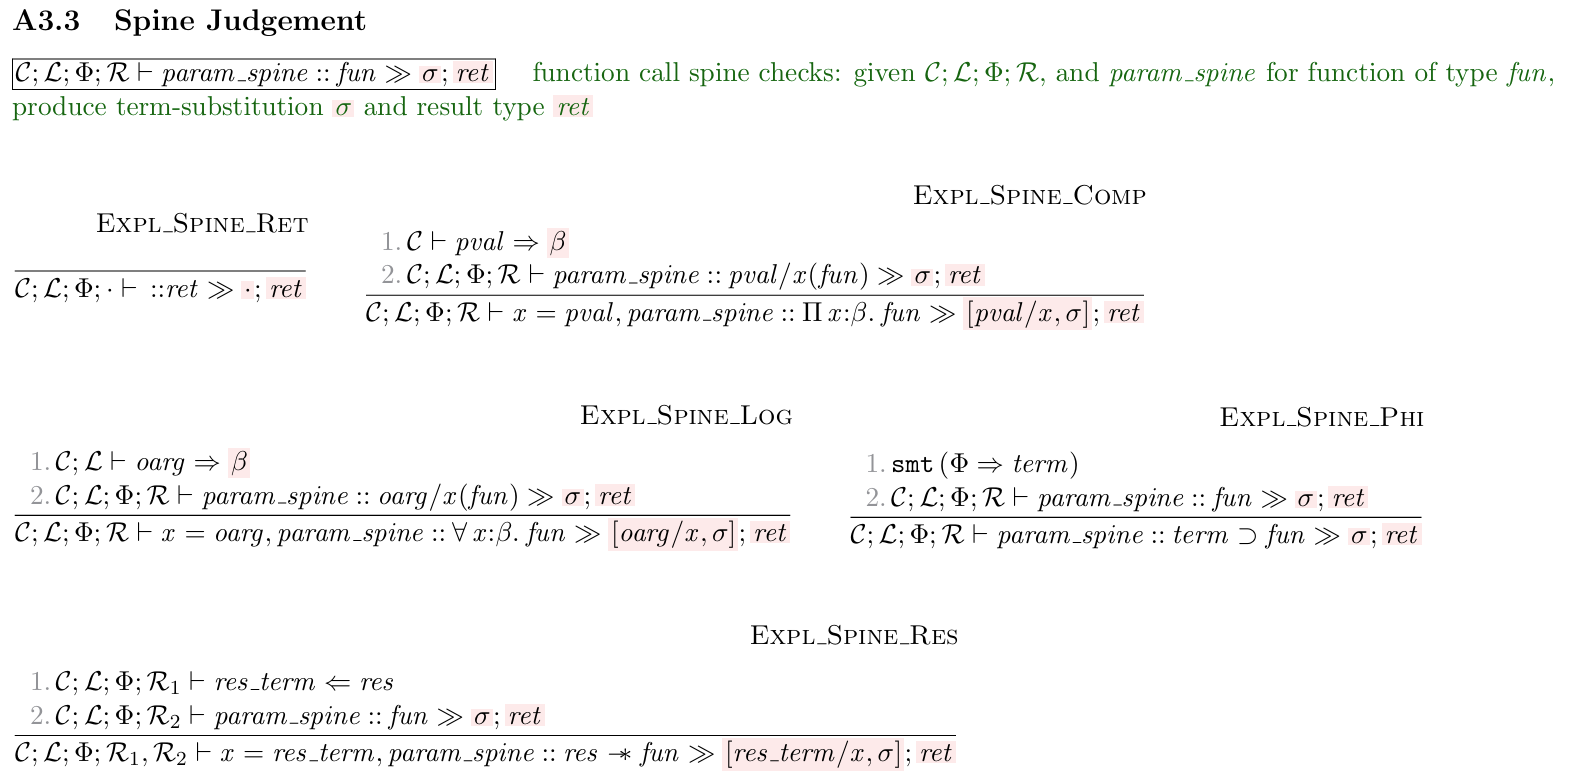
\includegraphics{figures/kernel-spine-typing}
    \caption{\kl{Kernel CN} typing rules for function
        spines.}\label{fig:typing-spine}
\end{figure*}

The judgement for typing spines is $\mathcal{C}; \mathcal{L}; \Phi ;
\mathcal{R} \vdash \mathit{param\_spine} \mathrel{{:}{:}} \mathit{fun} >\!\!>
\outpol{\sigma}; \outpol{ret}$, which means that given the contexts, a spine of
matched-up parameters and arguments and a function type, produce a substitution
$\sigma$ and a return type $\mathit{ret}$.

Function types are dependent over computational and logical (ghost) variables.
For notational convenience, I assume that the variables are the same as the
parameters in the spine. Typing these is done by substituting their
instantiation\sidenote{Remember that for \kl{kernel CN}, I assume all logical
(ghost) quantifiers are explicitly instantiated.} them into the type and typing
the rest of the spine. The substitution produced by this is extended with the
same.\sidenote{Building the substitution this way, rather than
`tail-recursively', made it easier to prove properties about it by induction
(\cref{sec:sub-ctxts}).}\label{sn:tail-rec-sub}. Constraints in types are
simply checked by the calling the SMT solver, and resources in types are
checked by splitting resource context, using one part to type the resource
term, and the other part to type the rest of the function type. Though these
types are not dependent over resources, the terms are, so this rule extends the
produced substitution with one for the resource too.

\section{Effectful values and expressions}

The spine typing is used in the rules for calling elaborated C function
\coreinline{ccall()}, and effectful Core procedures % chktex 36
\coreinline{pcall()}, in \cref{fig:typing-seq-expr-tval}. Both are % chktex 36
syntactically effectful sequenced expressions, typed with a judgement of the
form $\mathcal{C}; \mathcal{L}; \Phi; \mathcal{R} \vdash \mathit{seq\_expr}
\Rightarrow \outpol{ret}$, which says that given the contexts and an effectful
sequenced expression, synthesise a return type. Both lookup a function type for
the called function/procedure,\sidenote{\kl{CN} does not support
computed/indirect function calls, so I assume the callee has already been
resolved.} and simply produce the return type synthesised by the spine
judgement. This is also basically identical to how the top-level value
\coreinline{done<_>} is typed, with the main difference that (a) the judgement
$\mathcal{C}; \mathcal{L}; \Phi; \mathcal{R} \vdash \mathit{tval} \Leftarrow
\mathit{ret}$ is checking (b) the return type must be mapped to its dual
function type before using the spine judgement. Similar to the pure case, the
\coreinline{undef()} and \coreinline{error()} constructs % chktex 36 check
against any type if the constraint context is inconsistent.

\begin{figure*}[tp]
    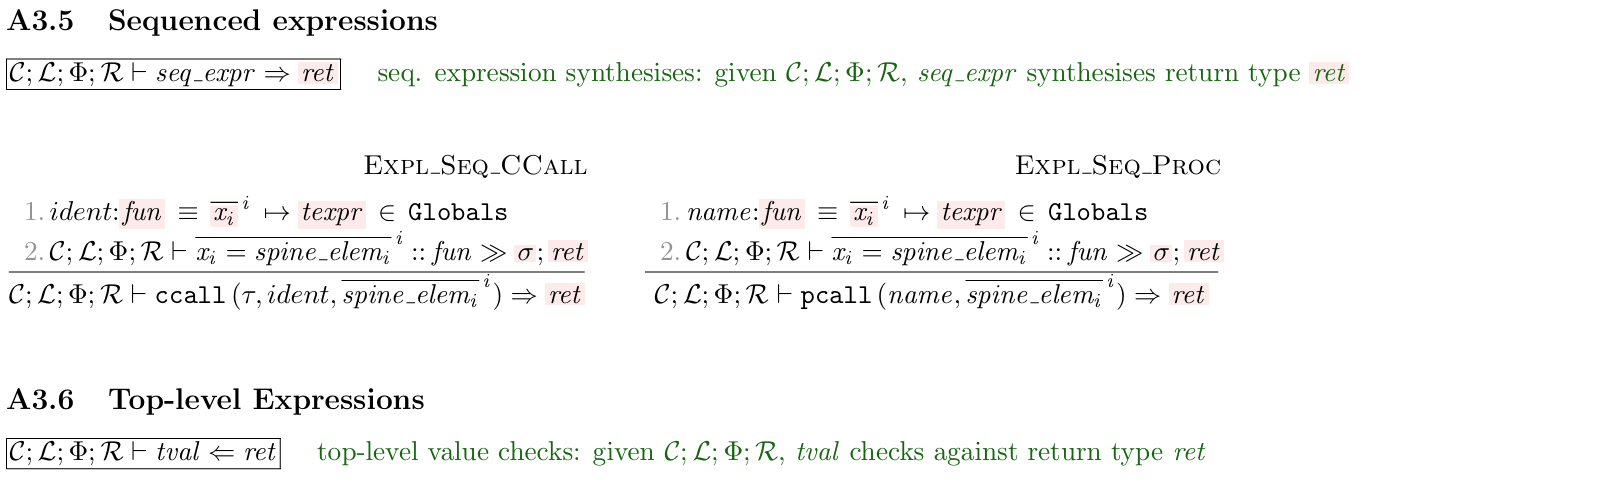
\includegraphics{figures/kernel-seq-expr-typing}
    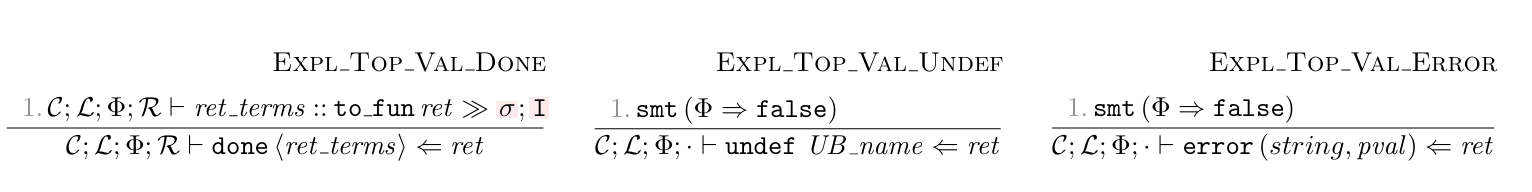
\includegraphics{figures/kernel-tval-typing}
    \caption{\kl{Kernel CN} typing rules for sequential expressions and top-level values.}\label{fig:typing-seq-expr-tval}
\end{figure*}

\section{Pattern matching}

Pattern matching is a surprisingly important crux of \kl{kernel CN}'s type
system because it \emph{is} the canal which directs a rich the grammar of
resource and return types into contexts. The judgement for this is
$\mathcal{C}; \mathcal{L}; \Phi \vdash \mathit{ret\_pat} {:} \mathit{ret}
\rightsquigarrow \outpol{\mathcal{C}'; \mathcal{L}'; \Phi'; \mathcal{R}'}$,
which says that given the contexts, a return pattern and a return type,
synthesise computational, logical, constraint and resource contexts.

Pattern matching for return types is complicated by the fact that they are
dependent on computational and logical (ghost) variables, and complicated
further by the fact that the computational values have their own patterns
(\cref{fig:typing-tpval-tpexpr}).

\begin{figure*}[tp]
    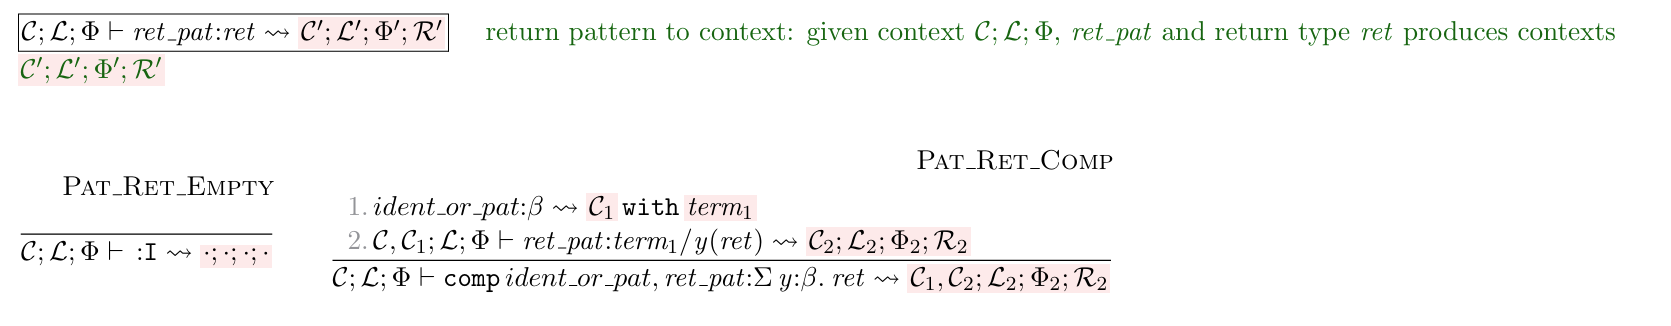
\includegraphics{figures/kernel-ret-pat-typing-1}
    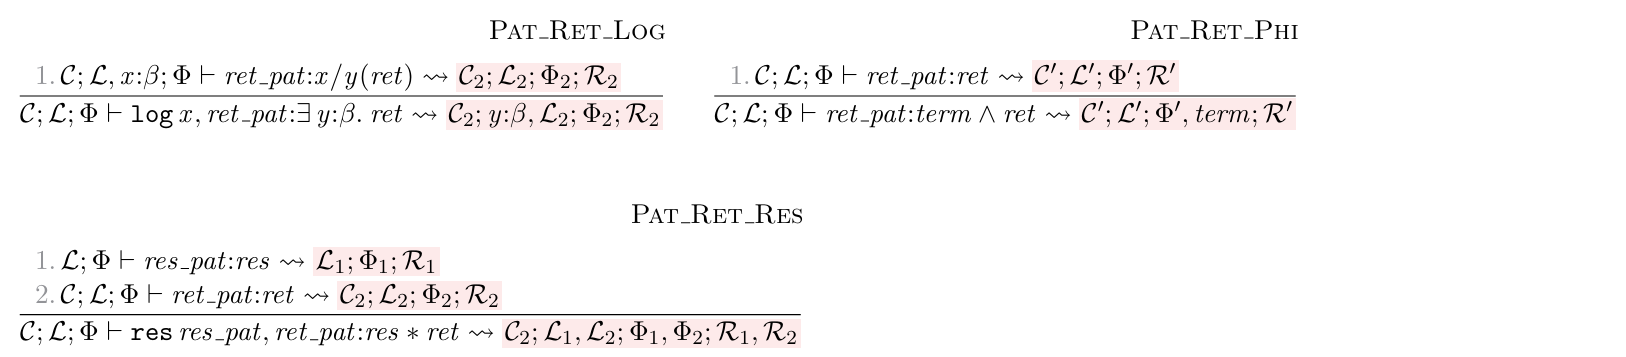
\includegraphics{figures/kernel-ret-pat-typing-2}
    \caption{\kl{Kernel CN} typing rules for pattern matching at return
        types.}\label{fig:typing-res-pat}
\end{figure*}

If both the head of the type and pattern are computational, the
\textsc{Pat\_Ret\_Comp} rule first uses the heads to synthesise a computational
context $\mathcal{C}_1$ and a represenative $\mathit{term}_1$ of the expected
shape. The former extends the input context, and the latter is substituted into
the the rest of the return type. After the remainder of the pattern is
converted into contexts, it is extended with $\mathcal{C}_1$.\sidenote{Similar
to what I mentioned in note~\ref{sn:tail-rec-sub} about substitution, I build
the contexts this way, rather than `tail-recursively', to make it easier to
prove properties about it by induction (\cref{sec:sub-ctxts}).}

If both the head of the return type and pattern are logical, then context is
extended with the pattern variable,\sidenote{\kl{CN} added support for
algebraic datatypes after I formalised \kl{kernel CN}
(\href{https://github.com/rems-project/cerberus/commit/0e5020732df2ec444ffa7a67abcc7c2c82904d24}{commit
0e50207}) and so and I did not formalise logical pattern matching; I would
formalise it identically to computational pattern matching.} and the same is
substituted into the rest of the return type. Similar to the computational
rule, the synthesised contexts is extended with the pattern variable.

Pattern matching for constraints simply adds the constraint to the contexts
synthesised by the rest of the return type for any pattern. And pattern
matching for resources similarly synthesises combines contexts from both the
resource type and pattern, and the rest of the return type and patterns.

This brings us on to how resource patterns synthesise contexts
(\cref{fig:typing-resp-pat}). The judgement for this is $\mathcal{L}; \Phi
\vdash \mathit{res\_pat}{:}\mathit{res} \rightsquigarrow \outpol{\mathcal{L}';
\Phi'; \mathcal{R}'}$, which means that given contexts,\sidenote{I abuse the
notation slightly and omit the computational context $\mathcal{C}$ because it
remains the same in all the rules.} a resource pattern and a type, synthesise
logical, constraint and resource contexts.

\begin{figure*}[tp]
    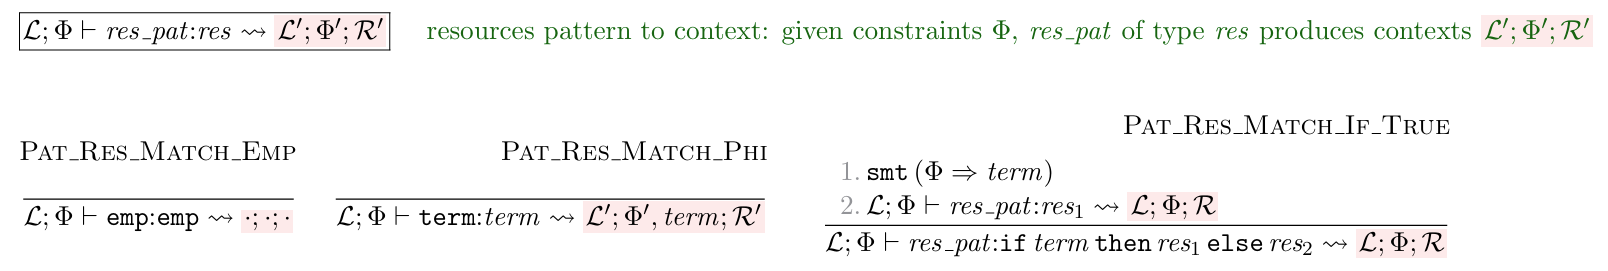
\includegraphics{figures/kernel-res-pat-typing-1}
    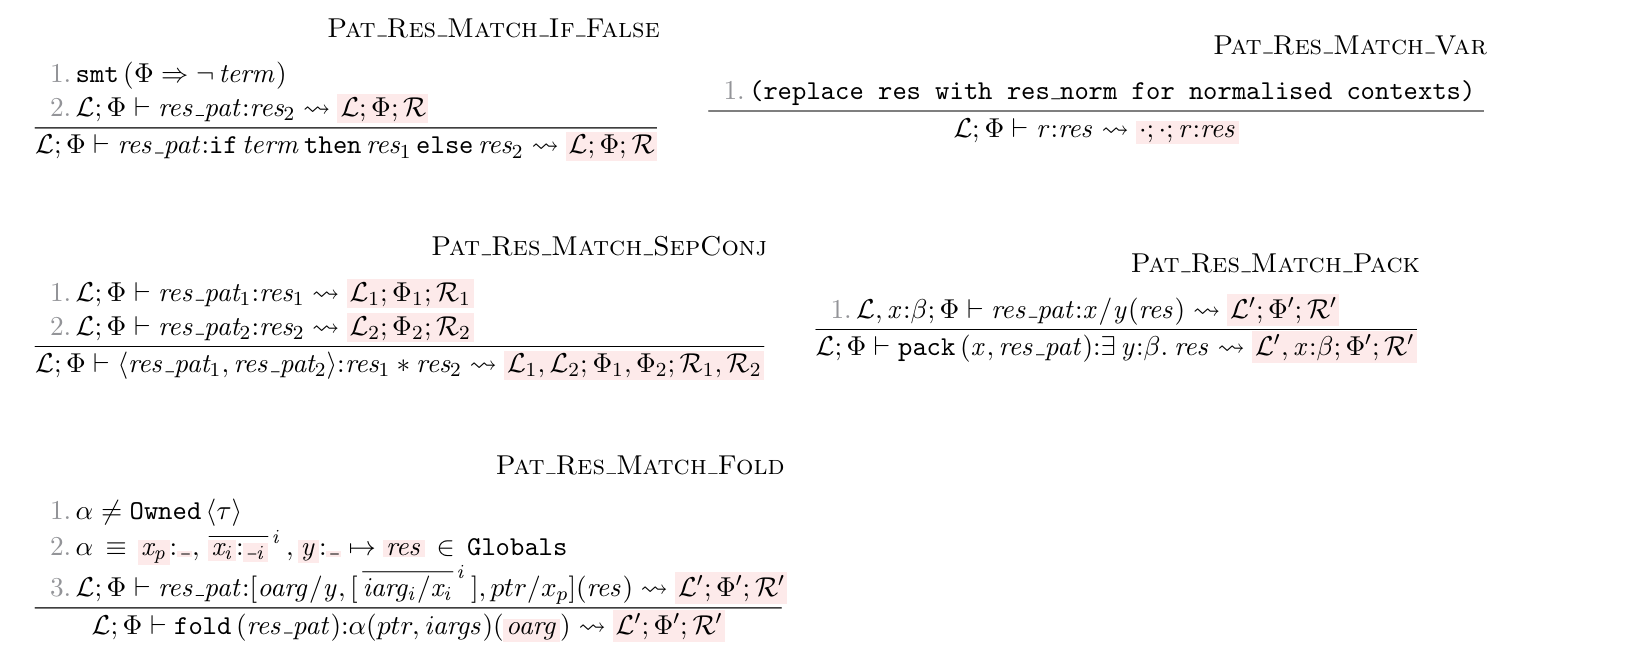
\includegraphics{figures/kernel-res-pat-typing-2}
    \caption{\kl{Kernel CN} typing rules for pattern matching at resource
        types.}\label{fig:typing-res-pat}
\end{figure*}

I am going to focus only on the rules for ordered-disjunctions and folds; the
rest are as expected. For the former, similar to its checking rule, its
condition or its negation must be proven, after which the corresponding branch
against is destructed on the same pattern; dual to its introduction by any
term, it can also be eliminated by any pattern. In the case of
\kl{under-determined} conditions, only the wildcard or the variable pattern
will match against the type. For the latter, the pattern only destructs when
the type is a predicate type and the nested pattern destructs against the
definition of that predicate (with the arguments substituted).

\section{Effectful top-level expressions}

With pattern matching in hand, I can explain the typing rules for effectful
top-level expressions (\cref{fig:typing-seq-texpr}). For space, I will
only talk about \coreinline{let} and \coreinline{run()} expressions, % chktex 36
the remaining rules are as one would expect presented in the appendix.

Top-level expressions are all checked, but the bound expression in the
\coreinline{let} is synthesised, so that the type can be used as part of
destructing the pattern it is bound against to synthesise extra contexts. Those
contexts are then appended to the existing one to check the body of the
\coreinline{let}. As for the \coreinline{run()} operator, the rule % chktex 36
looks up the function type belonging to the label being run, and then checks
that the spine satisfies that function type. Unlike the previous function call
operators, control flow does not return from a \coreinline{run()} % chktex 36
and so the type synthesised is expected to be false, and it checks against any
type.\sidenote{Need to update the rule.}

\begin{figure*}[tp]
    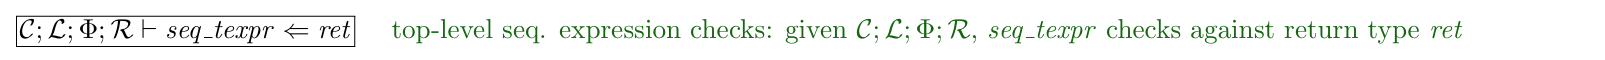
\includegraphics{figures/kernel-seq-texpr-typing-1}
    \begin{minipage}{0.7\textwidth}
        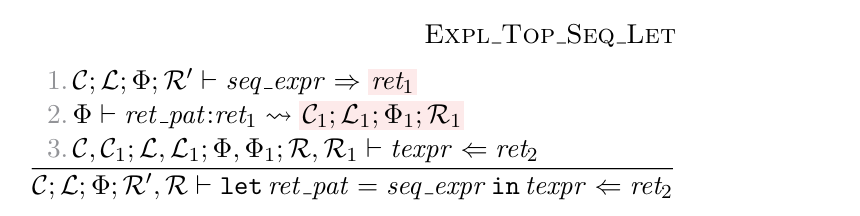
\includegraphics{figures/kernel-seq-texpr-typing-2}
    \end{minipage}
    \begin{minipage}{0.7\textwidth}
    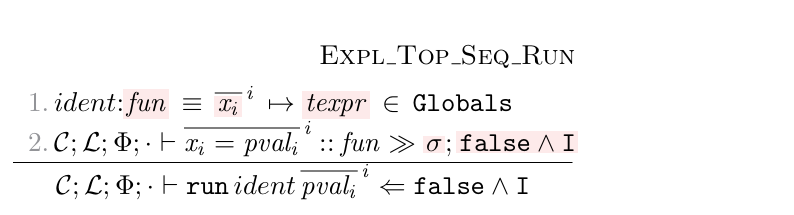
\includegraphics{figures/kernel-seq-texpr-typing-3}
    \end{minipage}
    \caption{Select \kl{Kernel CN} typing rules for effectful top-level
        expressions.}\label{fig:typing-seq-texpr}
\end{figure*}

\section{Elaboration}

Part of the \kl{Kernel CN} system also includes a specification for an
\emph{elaboration} system. At the time it was formalised, \kl{CN}
required users to manually fold and unfold predicates\sidenote{I should change
    the formalised grammar to use fold and unfold even though the terms CN used
we pack and unpack.}, but inferred indices for iterated predicates
automatically. Now, CN automatically folds and unfolds predicates but requires
users to state which indices are allowed to be moved in and out of any iterated
predicates in the context.\sidenote{See note~\ref{sn:inf-statics}.}
Instantiations for logical quantifiers were and continue to be inferred.

The goal of an elaboration pass over \kl{Kernel CN} is to take as an input a
well-formed program in \kl{ResCore} which has no explicit resources terms and
no instantiations for logical quantifiers on function calls, memory actions or
pointer operations, and to return the same program with the missing pieces
filled in, such that the above typing rules would pass if the program was
successfully elaborated, and fail if there was no elaboration possible.

I do not have a proof of these properties and so I cannot claim that the system
I am about to present meets the above goals. However, it is still useful to
present it, as it highlights some of the challenges in specifying such a system
in the first place; it also clarifies a few points about \kl{CN}'s
implementation (\cref{sec:restriction-branching}).

I shall only present a small slice of the elaboration to highlight the key
concepts, leaving the rest of the large system to the appendix. The main
judgement for synthesising a resource term and an instantiation for a logical
quantifier is $\Phi; \underline{\mathcal{R}} \vdash \mathtt{calc}\; y \;
\mathtt{using} \mathit{res} \rightsquigarrow \mathtt{bind}\;
\outpol{res\_bind}\; \mathtt{for} \outpol{res\_term} \; \mathtt{and} \;
\outpol{oarg} \dashv \outpol{\underline{\mathcal{R}'}}$
(\cref{fig:elab-res-oarg}). Given a constraint context, a resource context, an
output parameter, and a resource type, synthesise a series of bindings for an
output argument and resource term and which will result in the updated resource
context.

\begin{figure*}
    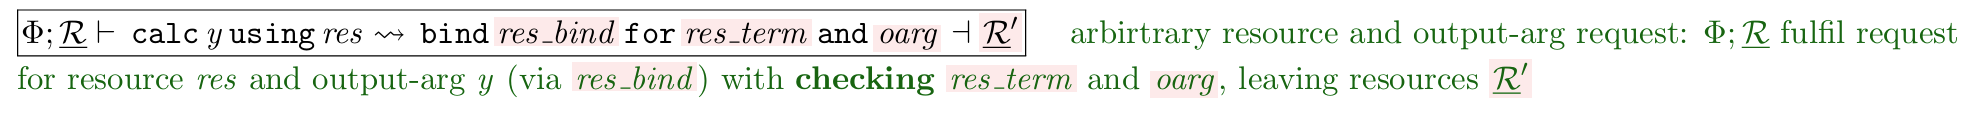
\includegraphics{figures/kernel-elab-calc-1}
    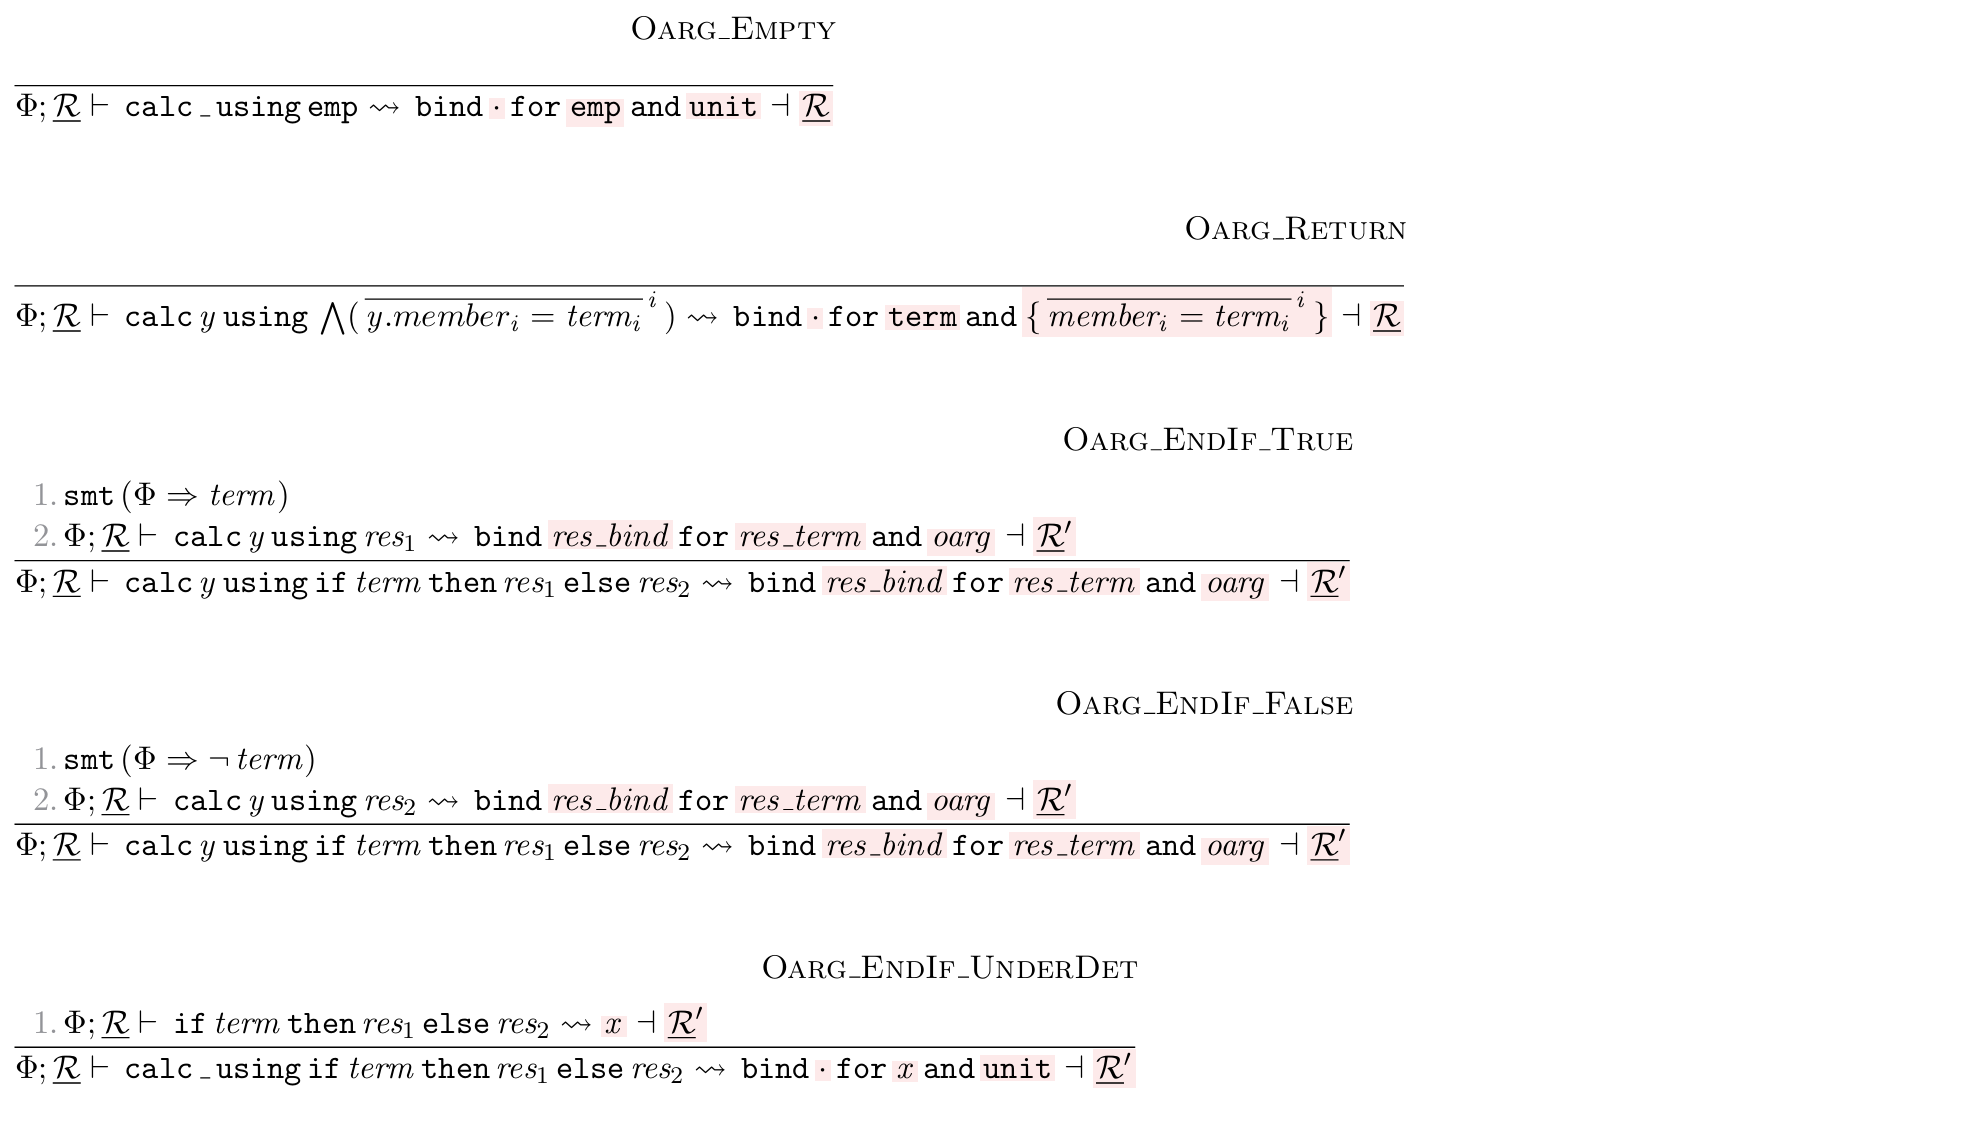
\includegraphics{figures/kernel-elab-calc-2}
    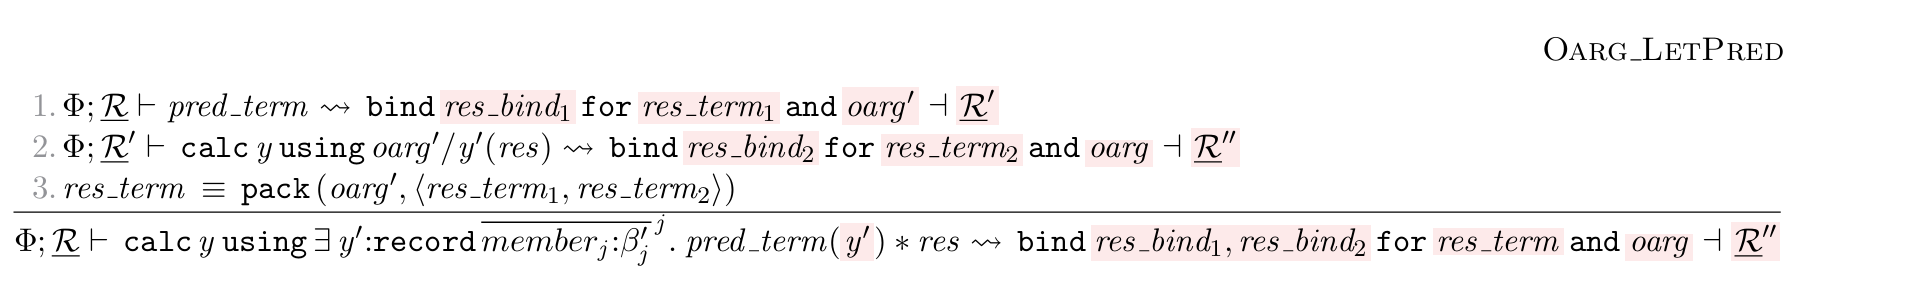
\includegraphics{figures/kernel-elab-calc-3}
    \caption{Select \kl{Kernel CN} rules for an elaboration pass which given
        contexts and a resource type, infers proof terms and logical quantifier
        instantiations satisfying those types.}\label{fig:elab-res-oarg}
\end{figure*}

\subsection{Normalised resource contexts}\label{sec:norm-ctxt-res}

One of the key restrictions I place to allow inference to be specified
relatively simply is that of a \intro{normalised} resource context, signified
with an underlined $\underline{\mathcal{R}}$, containing only normalised
resources types. A normalised resource is either an (iterated) predicate, or an
under-determined conditional resource. I call it normalised because (with the
appropriate terms and pattern-matching), any resource context can be
manipulated into such a normal form. This means it is simple to specify lookups
in the context: if I need $b \astRef{} c$ but the context has $\{\; x : a
\astRef b , y : c \astRef{} d \}$ then how should I proceed? Do I lookup $b$
and $c$ individually? Together? Swapped? How do I handle the case where one is
a sub-resource of a resource in the context? I avoid these questions and simply
require that other judgements which use resource lookup (all of them) simply
preserve normality as an invariant. This requires constructing rebindings of
existing terms (\cref{fig:res-bind-def}) to manipulate the context, carefully
retaining `leftover' resources from a lookup.

\begin{marginfigure}
    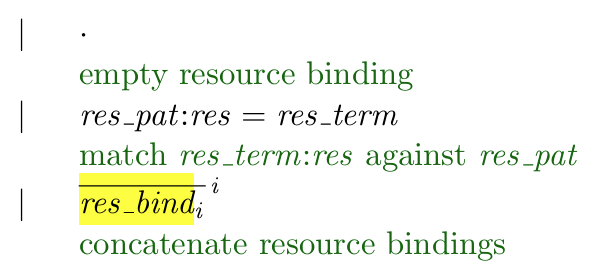
\includegraphics{figures/kernel-res-bind-def}
    \caption{\kl{Kernel CN} definition of resource bindings Note that these are
        only required in the presence of explicit resource terms, and as such
        are not necessary in \kl{CN}'s implementation.}\label{fig:res-bind-def}
\end{marginfigure}

\subsection{Synthesising resource terms and output arguments}

The judgement for synthesising resource terms and output arguments relies on
the fact that the more flexible \kl{kernel CN} types (\cref{fig:kernel-res})
have come from a translation (\cref{fig:pred-to-kernel}) of the intentionally
rigid surface syntax (\cref{sec:monadic-syntax}). Synthesising a term for
$\mathsf{emp}$ is simple and does not change the context, and the synthesised
output argument is just a dummy value.

Synthesising an output argument from equality constraints\sidenote{Should
update the rule to use a single one.} is just taking the right-hand-side of the
equality. Synthesising a resource term and an output argument for a
ordered-disjunction requires proving the condition or its negation, and then
synthesising the appropriate branch. For under-determined conditions, as
mentioned in~\nameref{subsec:checking-res-terms}, the term must be a variable
from the resource context whose type matches syntactically, modulo SMT
provability.

By construction, every existential quantifies over the output argument of
(iterated) predicates, and so synthesising a resource term and an output
argument for the \emph{whole} requires synthesising the output argument of the
(iterated) predicate. That it in turn, may require inferring an index to the
resource from an iterated version, which is handled by a separate judgement.
The inferred argument is substituted into the rest of the resource type to
infer another resource term and the originally requested output argument. The
synthesised resource term simply pairs and packs the aforementioned two, whilst
the synthesised output argument is the \emph{second} one (the first one was for
the existential).

\subsection{Synthesising indices for iterated predicates}\label{subsec:synth-indices}

Inferring indexes was possible, and relatively straightforward, because of the
requirement that every predicate had as its first input argument a pointer $p$,
and that every iteration over index $i$ of such predicates had as its first
argument $p +_\mathrm{ptr} i * \mathit{step}$ where $\mathit{step}$ is some
constant integer. Given these, inferring an index (for either
\coreinline{break}ing or \emph{glue}ing) reduced to $i = (p' - p) /
\mathit{step}$ where $p'$ is the pointer in the first argument of the request
predicate. This is made precise in \cref{fig:res-diff-break}.\sidenote{This
allows for empty iterated remainder: change it?}  The judgement $\Phi \vdash
\mathit{ident}{:}\underline{\mathit{res}} \mathbin{{-}?} \mathit{res\_req}
\rightsquigarrow \outpol{res\_diff}$ says that given constraint context, a
\kl{normalised} resource,\sidenote{Predicate (iterated) or an under-determined
ordered-disjunction.} and a request for a predicate (iterated), synthesise the
`difference' between the two. As shown in \cref{fig:res-diff-def}, the
`difference' can be of four sorts: no difference, exact match, subset match,
overlapping match and each requires slightly different handling (continue
search, stop search, bind remainder and stop search, bind remainder and
continue search respectively) from the lookup judgement (in appendix).

\begin{marginfigure}
    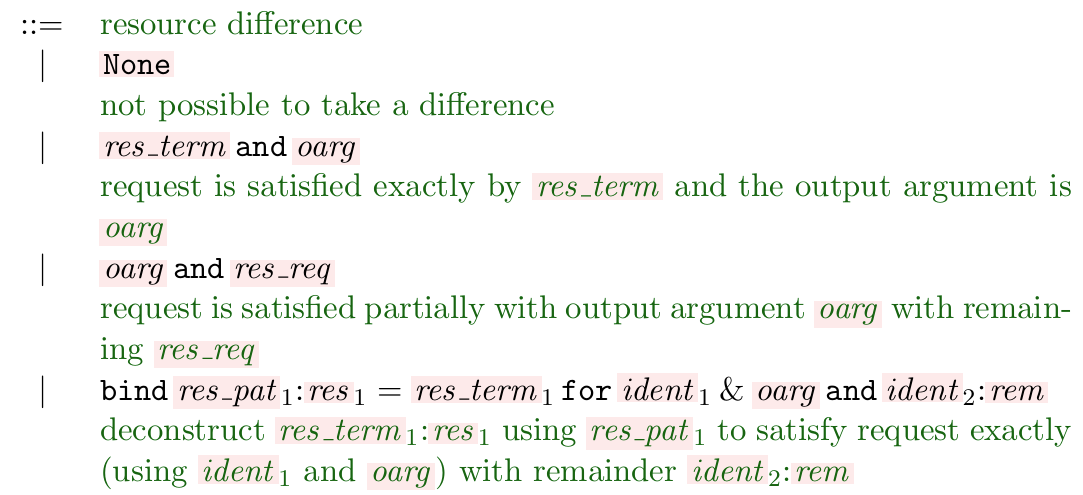
\includegraphics{figures/kernel-elab-res-diff-def}
    \caption{\kl{Kernel CN} definition of a `resource difference'. The second
        `and' needs to be changed to a `rem'.}\label{fig:res-diff-def}
\end{marginfigure}

\begin{figure*}[tp]
    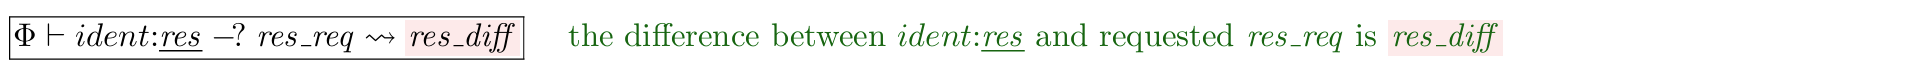
\includegraphics{figures/kernel-elab-diff-1}
    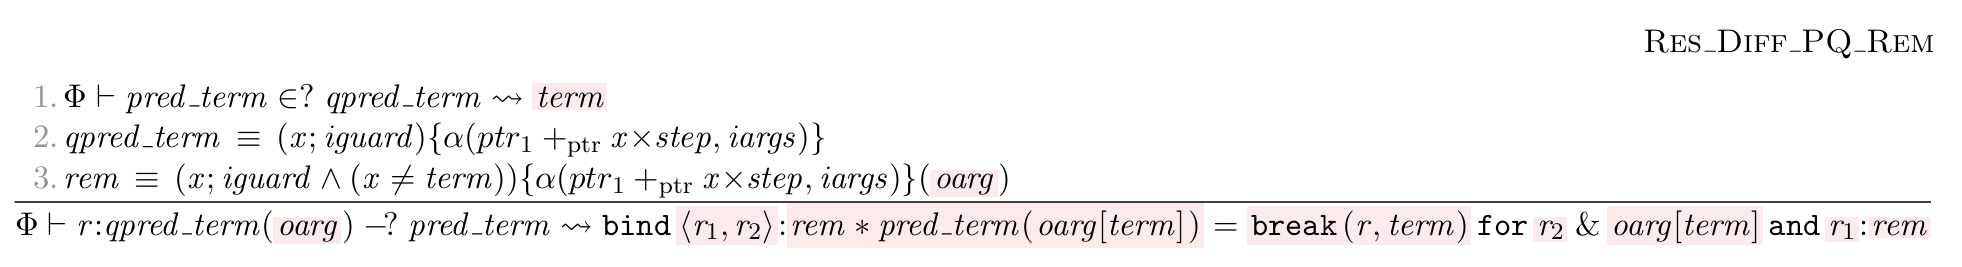
\includegraphics{figures/kernel-elab-diff-2}
    \caption{Select \kl{Kernel CN} elaboration rule for inferring indices and
        synthesising predicate operations.}\label{fig:res-diff-break}
\end{figure*}

\subsection{Using elaboration judgements}

It is important to note that the `calc' judgement synthesises a checking
resource term, and so care must be taken for it to be used in a checking
position. The main place this judgement is used however was for manually
folding predicates (\cref{fig:kernel-elab-fold}), which by accident of \kl{CN}'s
original implementation was in a synthesis position in the grammar rather than
a checking one (hence the type annotation on folding resource
terms,~\cref{subsec:synth-res-term}). The judgement is similar to a
synthesising typing judgement, but in addition to synthesising a return type,
it also synthesises a list of resource bindings to manipulate the context, and
an elaborated expression containing the fold resource term with several type
annotations to engineer into a synthesis form.

\begin{figure*}[tp]
    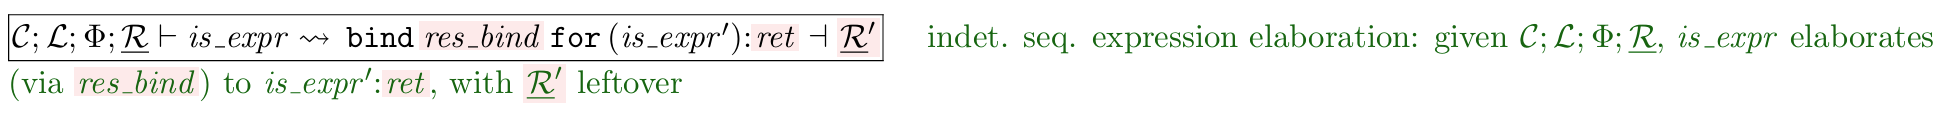
\includegraphics{figures/kernel-elab-fold-1}
    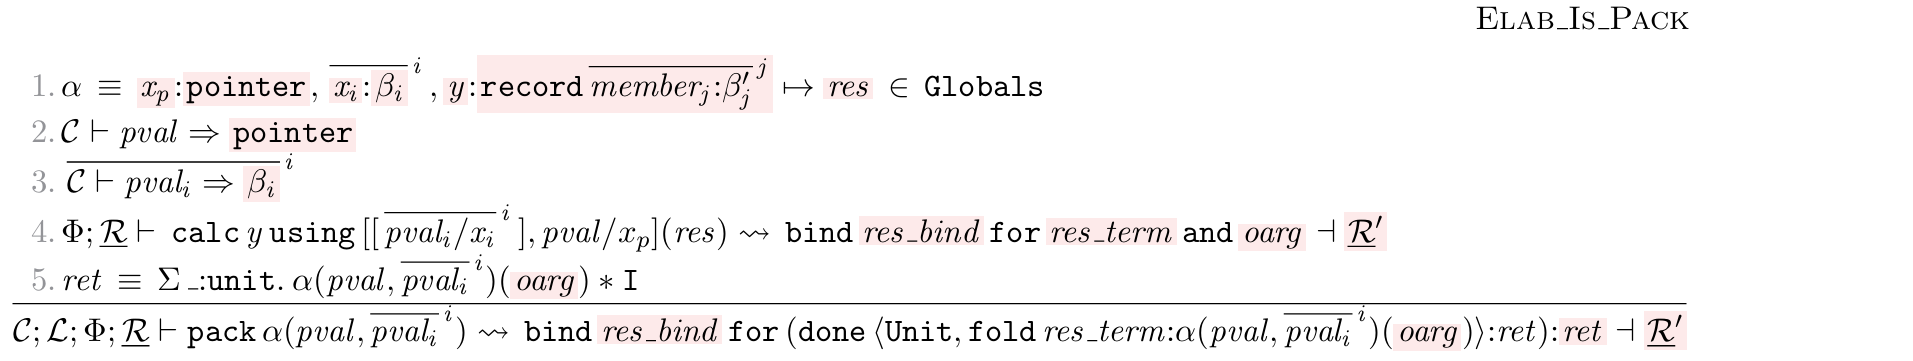
\includegraphics{figures/kernel-elab-fold-2}
    \caption{\kl{Kernel CN} elaboration rule for manually folding
        predicates.}\label{fig:kernel-elab-fold}
\end{figure*}

All other placements of resource terms only require (iterated) predicates, such
as memory actions like \coreinline{load} (\cref{fig:elab-action}) and spines
(\cref{fig:elab-spine}) for calls to elaborated C functions and Core
procedures. In these cases we see that the output argument is used only in
return types\sidenote{The synthesised return types are used in turn to
synthesise patterns to maintain the invariant that the resource context is
always normalised.} but that the resource terms (and the resource bindings
which precede it to manipulate the context into the right form for typing these
terms) are the main things elaborated into the program.

\begin{figure*}[tp]
    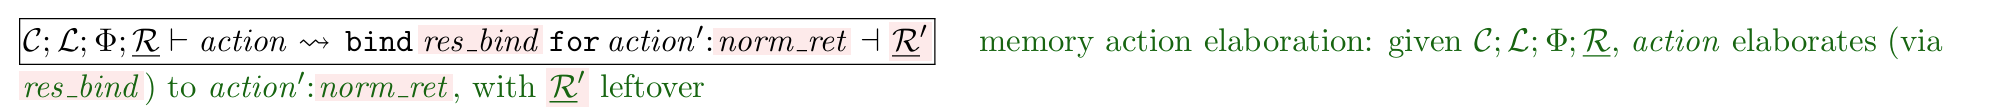
\includegraphics{figures/kernel-elab-action-1}
    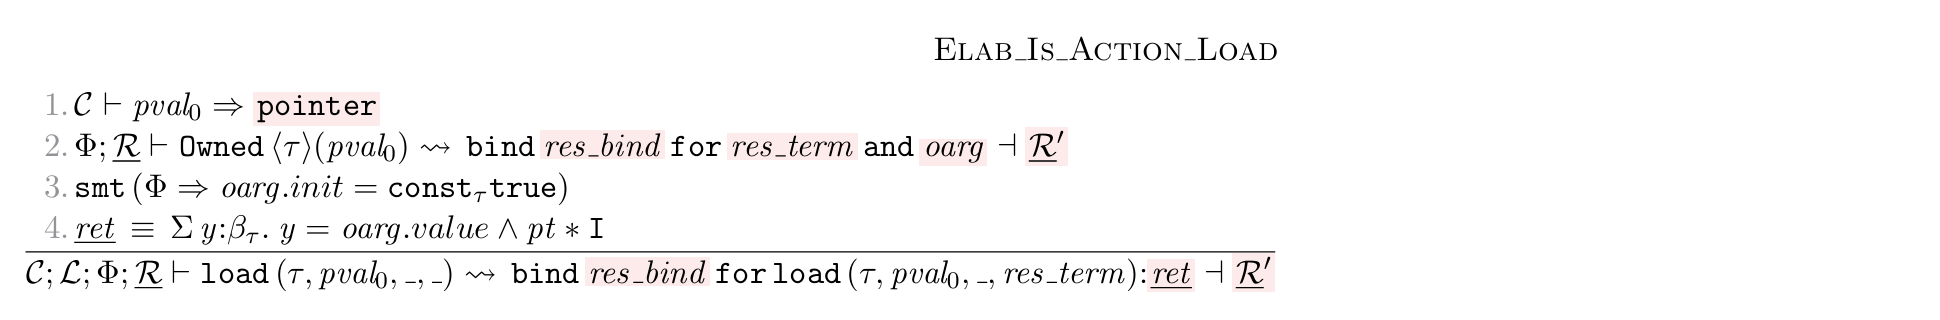
\includegraphics{figures/kernel-elab-action-2}
    \caption{Select \kl{Kernel CN} elaboration rule for memory
        actions.}\label{fig:elab-action}
\end{figure*}

\begin{figure*}[tp]
    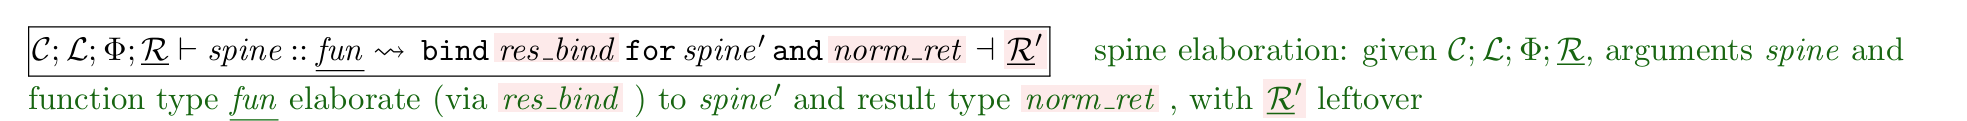
\includegraphics{figures/kernel-elab-spine-1}
    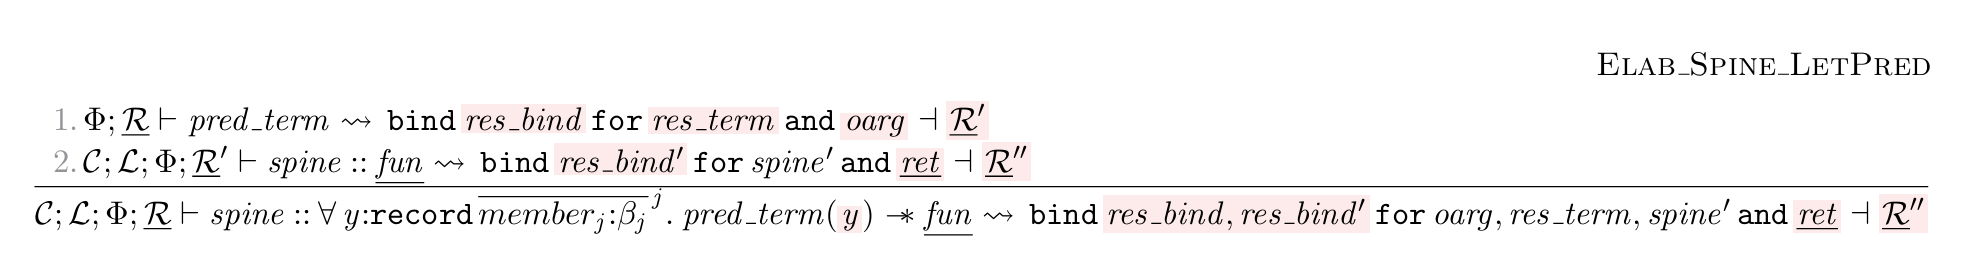
\includegraphics{figures/kernel-elab-spine-2}
    \caption{\kl{Kernel CN} elaboration rule for instantiating a logical
        quantifier when elaborating a function call spine.}\label{fig:elab-spine}
\end{figure*}

\chapter{Kernel CN:\ Proof of soundness}%
\label{chap:kernel-soundness}

To ensure that \kl{Kernel CN} had served as a useful formalisation for \kl{CN},
I proved that it was sound. The whole proof is large and in the appendix; In
this chapter, I will discuss the key definitions, lemmas and proof sketches. I
will first define an operational semantics for \kl{ResCore}, and then do a
straightforward, if not slightly tedious, syntactic proof of type
safety.\sidenote{The continuation-like behaviour of the \coreinline{run()} % chktex 36
and \coreinline{save()} operators make it more challenging to prove % chktex 36
soundness in a denotational manner.} This suffices because \kl{ResCore} is a
first-order language, and all functions and labels are annotated with the
correct type,  despite the presence of linear types, which usually require
logical relation methods.

The proof is split up into three smaller proofs: a joint
progress-and-type-preservation proof for resource term reduction, a progress
theorem, and a type-preservation theorem.

The definitions and lemmas of note in this proof are (a) the careful definition
of substitution, and its accompanying substitution lemma (b) the novel
structure of the heap, which is unusual in that is essentially just separation
logic predicate (c) the interaction between the resource terms and heaps.

\section{Substitution and contexts}\label{sec:sub-ctxts}

The first three rules for typing substitutions (\cref{fig:soundness-sub}) are
simple enough: the empty substitution represents the empty context, a
computational or logical substitution requires the substituted value to be well
typed, and same for the resource term. However, because resource terms and
types can depend on the first two, scoping needs to be handled carefully,
so resource types in a substitution may only mention variables
either in the contexts on the left of the turnstile, or the computational
and logical context in the substitution type. This makes it easier to decompose
substitutions into valid parts, each of which can be applied sequentially but
still produce a meaningful results (because of the dependent types,
substitutions may be telescoping, so need not commute). Hence, the
\textsc{Sub\_Chk\_Concat} rule checks not only the first half $\psi$ of the
substitution against half the context, but checks the second half
\emph{substituted} against second half of the context \emph{substituted}, to
eliminate any mention of variables from $\mathcal{C}_1$ and $\mathcal{L}_1$ in
$\mathcal{R}'_2$.

\begin{figure*}[tp]
    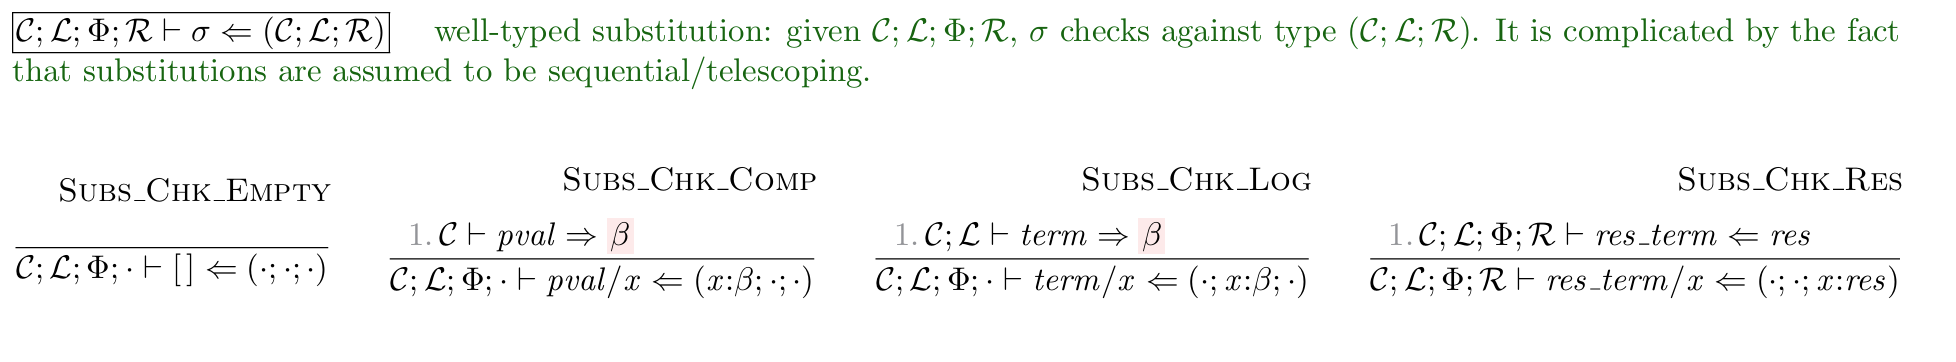
\includegraphics{figures/kernel-soundness-sub-1}
    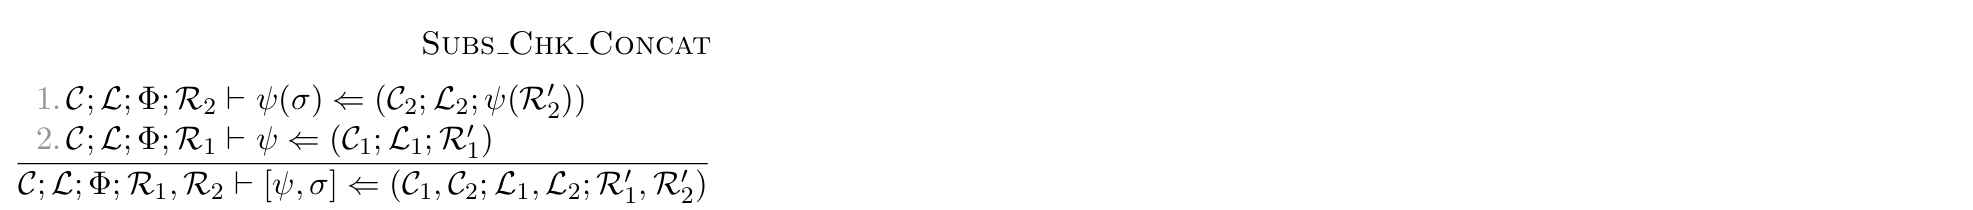
\includegraphics{figures/kernel-soundness-sub-2}
    \caption{\kl{Kernel CN} substitution typing}\label{fig:soundness-sub}
\end{figure*}

In the appendix, I use this definition to prove lemmas such as substitution
preserves SMT results and that substitutions can be split up (linearity means
this property is not completely trivial). The key lemma is the substitution
lemma stated below.

\begin{lemma}[Substitution lemma]
If $\mathcal{C}'    \mathcal{L}'  ;  \Phi  ;  \mathcal{R}'  \vdash  J$,
then $ \forall \ \mathcal{C}, \mathcal{L}, \mathcal{R}, \sigma.\
\left( \mathcal{C}    \mathcal{L}  ;  \sigma  (  \mathrm{ \Phi }  )  ;
\mathcal{R}  \vdash  \sigma  \Leftarrow  (  \mathcal{C}'  ;  \mathcal{L}'  ;
\mathcal{R}'  ) \right)  \Rightarrow \allowbreak
\mathcal{C}    \mathcal{L}  ;  \sigma  (  \Phi  )  ;  \mathcal{R}  \vdash  \sigma ( J ) $.
\\[\baselineskip]
If a judgement holds under some context, and the context is the type of
a substitution in \emph{another} context, then the judgement is also holds in
that other context substituted appropriately.
\\[\baselineskip]
Since $\Phi$ is scoped to $\mathcal{C}' ;
\mathcal{L}'$, we must substitute over it as well as all the usual suspects on
the right.\sidenote{I think this slightly off, $\mathcal{R}'$ is scoped the
same too and should need substituting as well.}
\\[\baselineskip]
Substitution of contexts is defined by substituting over each constraint in
$\Phi$. As a result, $\sigma (\Phi_1, \Phi_2) = \sigma (\Phi_1) , \sigma (\Phi_2) $,
and if $\sigma (\Phi) =  \Phi'_1 , \Phi'_2$ then $\exists \Phi_1,  \Phi_2 . \:
\sigma (\Phi_1, \Phi_2)   = \sigma (\Phi_1), \sigma (\Phi_2)$.
\end{lemma}

\paragraph{Proof sketch.} Full proof in the appendix. Induction over the typing
judgements. There are four parts to this proof.
\begin{itemize}
\item \textbf{Variable rules.} Repeatedly invert the substitution typing
    assumption until the variable used in the context appears, and then
    use the equational properties of substitution and the assumptions
    to prove the goal.
\item \textsc{Expl\_Top\_Val\_Done}. $\mathtt{to\_fun}$ commutes with
    substitution, but leaves terms unchanged, so induction proceeds
    straightforwardly.
\item \textbf{Context change rules.} Split up substitutions as required by the
    restrictions on the resource context. If a rule uses the SMT judgement, use
    the substitution preserves SMT results lemma.
\item \textbf{Remaining rules}. Straightforward induction.
\end{itemize}

\section{Heaps and their types}\label{sec:heap-types}

Heaps in the operational semantics are, slightly unusually, tree-shaped
collections of predicates (\cref{fig:kernel-heap-def}). The leaves of the tree
are the built-in ownership and allocation predicates; the branches of the heap
are predicates tagged with their definition (a resource value of the type of
the predicate body) and a sub-heap (of the resources used by the definition).

\begin{marginfigure}
    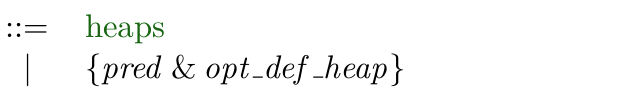
\includegraphics{figures/kernel-dynamics-heap-1}
    
\includegraphics{figures/kernel-dynamics-heap-2}
    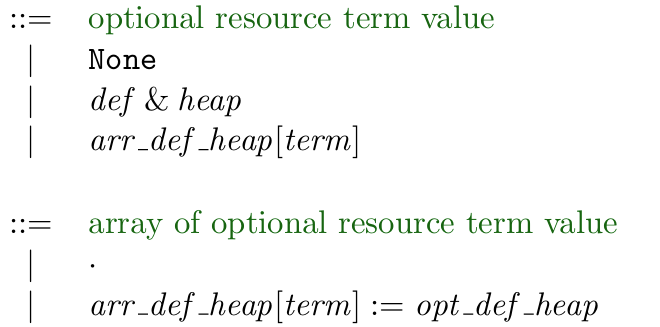
\includegraphics{figures/kernel-dynamics-heap-3}
    \caption{\kl{ResCore} dynamics heap definition.}\label{fig:kernel-heap-def}
\end{marginfigure}

Resource \emph{values} are the subset of resource terms which cannot reduce
further (\cref{fig:kernel-res-val-def}). This is to capture the idea that
predicates encapsulate their contents until opened.

\begin{marginfigure}
    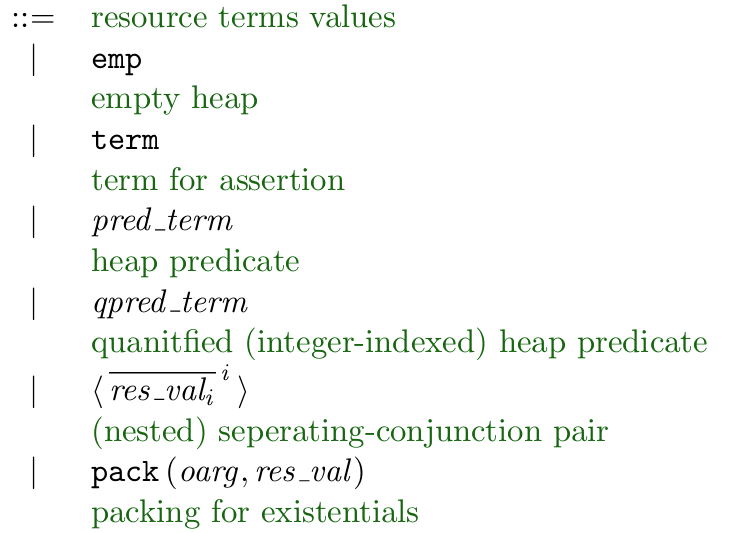
\includegraphics{figures/kernel-dynamics-res-val}
    \caption{\kl{ResCore} resource \emph{values} (subset of terms).}\label{fig:kernel-res-val-def}
\end{marginfigure}

This means that, in the dynamic semantics, folding (and via pattern matching,
unfolding) predicates \emph{affect the shape of the heap}
(\cref{fig:kernel-fold-unfold}). In the unfold rule, the nested definition is
used to destruct the rest of the pattern into a substitution, and the heap is
extended with the sub-heap associated with those values.

\begin{marginfigure}
    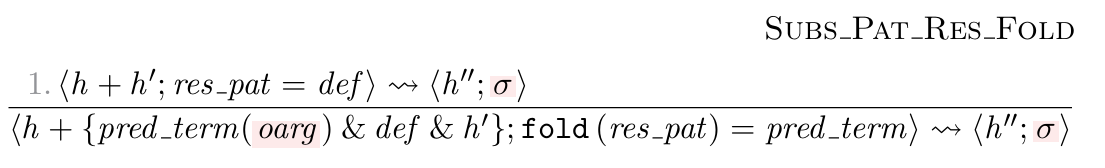
\includegraphics{figures/kernel-dynamics-unfold}
    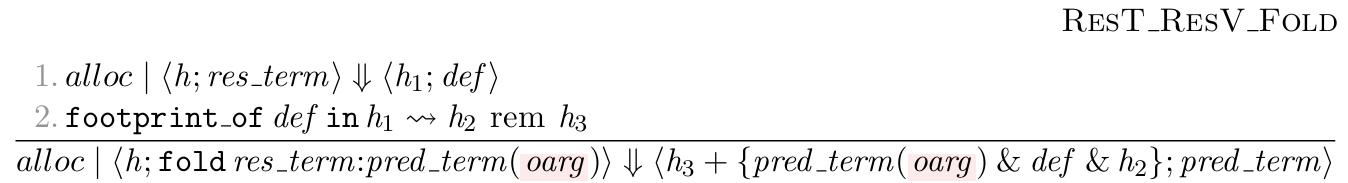
\includegraphics{figures/kernel-dynamics-fold}
    \caption{\kl{ResCore} dynamics for folding and unfolding
        predicates.}\label{fig:kernel-fold-unfold}
\end{marginfigure}

In the fold rule, the inverse happens, which requires splitting a heap into the
\emph{footprint} of some resource values, and the remainder
(\cref{fig:kernel-footprint}). I define the footprint of a resource value as
the sub-heap containing the (iterated) predicates referred to in said value.

\begin{figure*}
    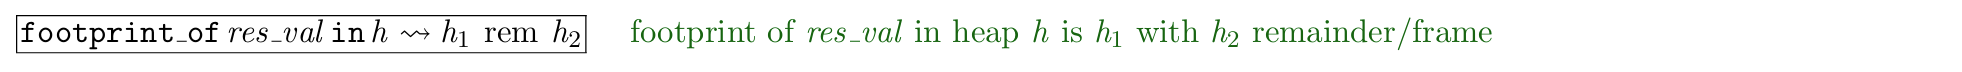
\includegraphics{figures/kernel-dynamics-footprint-1}
    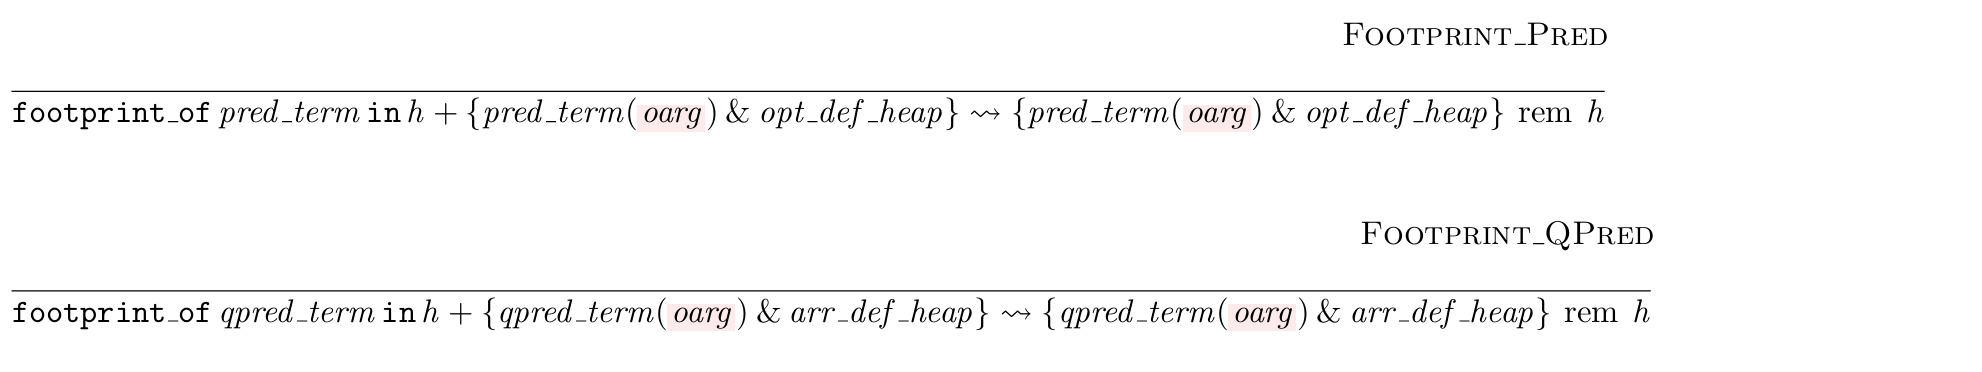
\includegraphics{figures/kernel-dynamics-footprint-2}
    \caption{\kl{ResCore} dynamics definition of a footprint of a resource
        value in a heap.}\label{fig:kernel-footprint}
\end{figure*}

I defined both the pattern matching and the resource term reduction dynamic
semantics in a big-step style; this makes the definition of both more concise,
at the cost of intertwining the usually separate proofs of progress and type
preservations for resource term reduction.

The final definition required for the proof is that of the type of a heap. The
type of a heap is a \kl{normalised resource} context
(\cref{sec:norm-ctxt-res}); the rules for these are straightforward
(\cref{fig:kernel-heap-typing}), except the fact a heap with a folded predicate
requires there exists a context for which the resource value $[[ def ]]$ and
$[[ heap ]]$ is well-typed. This becomes necessary for proving the progress of
pattern-matching for the whole of the annotated and let-normalised Core.

\begin{figure*}
    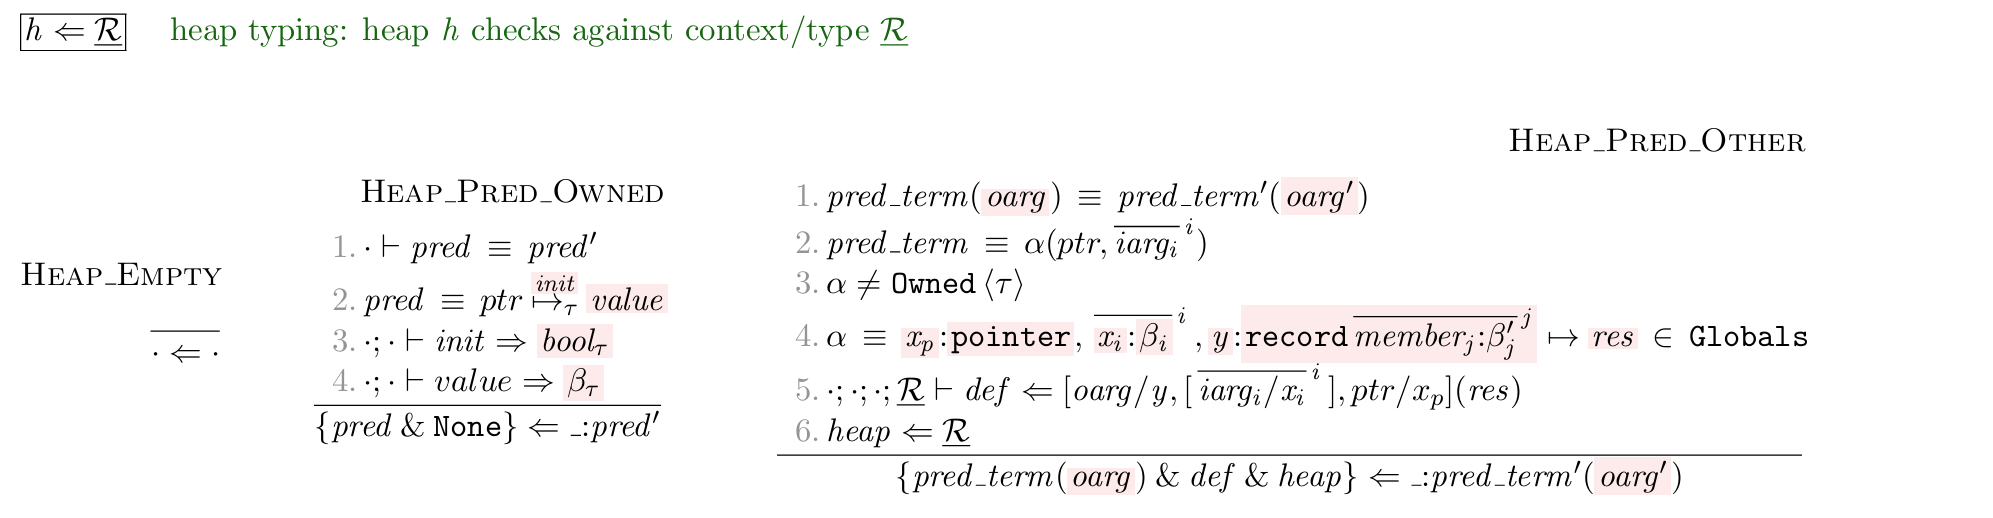
\includegraphics{figures/kernel-heap-typing}
    \caption{Select typing rules for heaps.}\label{fig:kernel-heap-typing}
\end{figure*}

As with elaboration, using normalised resource contexts does not restrict the
generality of progress and type preservations theorems.This is because of the
following lemma: if a well-typed resource term is closed, then the context in
which it is well-typed must normalised (formal definition and proof in the
appendix). We now have all the ingredients to state and sketch a proof for the
progress and type preservation for resource terms.

\begin{theorem}[Progress and type preservation for resource terms]
For all closed resource terms ($[[ res\_term ]]$) which type check or
synthesise ($[[ cdot ; cdot ; N ; nR |- res\_term <= res ]]$) and all well-typed
heaps ($[[ N |- h <= nR ]]$) there exists a resource value ($[[ res\_val ]]$),
context ($[[ nR' ]]$) and heap ($[[ h' ]]$), such that: the value is
well-typed ($[[ cdot ; cdot ; N ; nR' |- res\_val <= res ]]$); the heap is
well-typed ($[[ N |- h' <= nR' ]]$); for all frame-heaps ($[[ f ]]$), the
resource term reduces to the resource value without affecting the frame-heap
($[[ < h + f ; res\_term > ||v < h' + f ; res\_val > ]]$).
\end{theorem}

\paragraph{Proof sketch.} Full proof in the appendix. Induction on the resource
term typing assumption. The type dictates the value and context, the latter of
which dictates the shape of the heap; all of this relies heavily on a few
inversion lemmas. The existential is necessary later for proving well-typed
values pattern pattern match successfully, where it is used as a witness when
proving heap typing for folded predicates. The frame heap $f$ is necessary later
for

\section{Soundness}

The configuration for the operational semantics is a pair of a heap and a
ResCore program. As one might expect, proving progress requires well-typed
patterns successfully produce substitutions. I assume that all computational
patterns are exhaustive, because if they are not, this is a bug in Cerberus.
Proving well-typed patterns successfully produce substitutions is complicated
by two things, the solution to which requires the introduction of a relation on
SMT terms and resource types, $[[ N |- res \~ res' ]]$ (to be read ``under
constraints $[[ N ]]$, $[[ res ]]$ is related to $[[ res' ]]$'').

The first is that the constraint term generated when typing a computational
pattern (this is required to record, in the constraint context, which branch
the type system is assuming it is in) is not exactly equal to the values it can
match in the operational semantics (nor would we want it to be: the pattern $[[
Cons ( x1 , x2 ) ]]$ should match the value $[[ Cons ( pval1 , Cons ( pval21 ,
Nil base\_type ( ) ) ) ]]$). Hence, we must weaken the notion of equality on
types to $[[ \~ ]]$ relatedness, which links the two, so that during the proof,
we can substitute the constraint term $[[ x1 cons x2 ]]$ at the type-level, and
maintain a link to the corresponding value.

The second is that the conditions of related ordered-disjunctions must remain
SMT-equivalent (with reference to a constraint context), so that pattern-match
typing and resource term typing are consistent.

\begin{theorem}[Progress for the annotated and let-normalised Core]
If a top-level expression ($[[ texpr ]]$) is well-typed
($[[ cdot ; cdot ; N ; nR |- texpr <= ret ]]$) and all computational patterns
in it are exhaustive, then either it is a value ($[[ tval ]]$), or it is
unreachable, or for all heaps ($[[ h ]]$), if the heap is well-typed
($[[ N |- h <= nR ]]$) then there exists another heap ($[[ h' ]]$) and expression
($[[ texpr' ]]$) which is stepped to ($[[ < h ; texpr > --> < h' ; texpr' > ]]$)
in the operational semantics.
\end{theorem}
\paragraph{Proof sketch.} Induction over the typing assumption. Full proof in
appendix.

Moving on to type preservation, a few things are noteworthy about its proof.

First is that a frame-heap has to be explicitly passed around.  Whilst this is
inconvenient, it becomes necessary in the \textsc{Expl\_Top\_Seq\_LetT} case.

Second is in the lemma~\nameref{subsec:wt_values_pat_match}.
There are two substitutions at play here. As an example, let
the value being matched be $[[ Cons ( Unit , Nil unit ( ) ) , ret\_terms ]]$ and
the pattern be $[[ comp Cons ( x1 : unit , x2 : list unit ) , ret\_pat ]]$.
For the return type $[[ sigma y : list unit . ret ]]$, the type-level
substitution will be $[[ Cons ( x1 , x2 ) / y ( ret )]]$.  However, at the
term-level, the substitution will be $[[ [ Unit / x1 , Nil unit ( ) / x2 ] ]]$.
\emph{Bridging this difference is the main reason for the $[[ ~ ]]$ relation}
(the other is the use of $[[ to\_fun ret ]]$).  \emph{The type-level substitution
is open}, and only makes sense with respect to the variables introduced in the
pattern-match.

Lastly, we gather constraints throughout the proof, since these are accumulated
by the typing rules, during pattern-matching, case and if. Given the constraint
context is always well-formed
% VIP related (w.r.t.~to the initial logical variable context $[[ L0 ]] = [[ allocv : id\_map ]]$), this means that after substituting in the
allocation history, all the constraints involve no variables
% VIP related (hence the substitutions in \textsc{Heap\_Ty} and \textsc{Alloc\_Ty})
, and so will be trivially decidable.

\begin{theorem}[Type preservation for the annotated and let-normalised Core]
For all closed and well-typed top-level expressions
($[[ cdot ; cdot ; N ; nR |- texpr <= ret ]]$),
well typed heaps ($[[ N |- h <= nR ]]$),
frame-heaps ($[[ f ]]$),
new heaps ($[[ heap ]]$),
and new top-level expressions ($[[ texpr' ]]$),
which are connected by a step in the operational semantics
($[[ < h + f ; texpr > -->  < heap ; texpr' > ]]$),
if all top-level functions are annotated correctly,
there exists a constraint context ($[[ N' ]]$),
sub-heap ($[[ h' ]]$),
and resource context ($[[ nR' ]]$),
such that the constraint context is $[[ N ]]$ extended,
the frame is unaffected ($[[ heap ]] = [[ h' + f ]]$),
the sub-heap is well-typed ($[[ N' |- h' <= nR' ]]$),
and the top-level expression too
($[[ cdot ; cdot ; N' ; nR' |- texpr' <= ret ]]$).
\end{theorem}

\paragraph{Proof sketch.} Induction over the typing assumption. Full proof in
appendix.

\chapter{Informing implementation discussions}\label{chap:inform-impl}

In the early stages, \kl{CN} was implemented by Christopher Pulte and Thomas
Sewell, based on sketches by Neel Krishnaswami. I started formalising
\kl{Kernel CN} much later, and benefited by the clarity of having an
implementations and implementers to which and whom I could refer in moments of
confusion.

However, this mode of development means that there were \emph{many} design
decisions made in a rather conservative context, because the programming was
always of a system which was being defined along the way, rather than a
well-understood pre-existing one. Extensions to syntax and inference were
always the minimum required for verifying the pKVM buddy allocator, lest
performance and inference suffer greatly, rather than ones based on a strong
formal and holistic consideration of the constructs and interactions at play.

As such, there are several restrictions in the implementation, which with the
benefit of hindsight and formalisation, are completely unnecessary, but persist
as technical debt. This chapter list a few of these, and explains how the
formalisation brings much needed clarity to many questions around the
implementation.

\url{https://github.com/rems-project/cerberus/labels/language}
\url{https://github.com/rems-project/cerberus/labels/resource\%20reasoning}

\section{Supporting partially initialised reads of structs/unions}

So far in working on verifying the buddy allocator, writing a tutorial and
working with our industry partners, no code has needed to ability to read a
partially (including completely) uninitialised struct/union, and any valid code
which does this would have to simply ignore that result. The \kl{UB} only comes
when one tries to read an uninitialised primitive type member of the
struct/union from that earlier read.

Because we can decompose ownership of a struct into its fields, and track the
initialised status of those individually (perhaps verbosely for large structs),
it does not seems like we lose much in expressiveness in forbidding this. The
only valid code that would be additionally rejected if this was forbidden in
the type system would be a reads a partially initialised struct followed by a
call to a function which reads only the initialised fields. And in such
instances, it seems likely that the code could be refactored to only pass the
initialised fields, or a pointer with the appropriate precondition to only read
the initialised fields.

Although we wish to verify C code as is, because programmers need to change the
``code'' to write annotations anyway, such small, rare and easy to explain
refactors are a worthwhile trade-off if it makes the design and implementation
of \kl{CN} simpler. The book-keeping for tracking initialised status in
symbolic terms, rather than in a flag the name of a predicate, adds a
non-trivial amount of noise to formalisation and would do the same in the
implementation.

And when we think about the potential origins of allowing such behaviour.
Perhaps such an allowance simplifies data-flow analysis inside a compiler, so
that it may safely ignore the values resulting from a load of partially
uninitialised loads of a of struct, so long as none of the fields are accessed.
It seems hard to think of a case for this allowance motivate by performance or
programmer ergonomics, and so the experience from formalising this suggests
that the current implementation of \kl{CN}, which does not allow loads from
partially (including completely) uninitialised structs, can and will remain
expressive enough for all of its use cases.

\section{Auto unfolding scheme for logical functions}\label{sec:auto-unfold-functions}

\url{https://github.com/rems-project/cerberus/issues/483}

One the strange parts of working with \kl{CN} is the predicate definitions are
automatically unfolded but not logical functions, even though both may be
recursive. As such there is separate and cumbersome annotation to manually
unfold a function.

The way the implementation determines whether or not to unfold a predicate is
to always unfold it if there is no top-level if, or to check if the condition
or its negation can be proven before unfolding the corresponding branch.

However, with the benefit of the formalisation, we can see that those are
actually two orthogonal questions, which happen to be tied together because of
historical reasons. In the formalisation (\cref{fig:typing-res-pat}), including
the elaboration rules (\cref{fig:kernel-elab-fold}),  we can see that (un)folding % chktex 36
predicates does not require calling the SMT solver, but determining which
branch of an ordered-disjunction to check does.

So not only does this suggest loosening the restrictions on branching in
predicate definitions (\cref{sec:restriction-branching}), it also suggests that
the general approach of ``unfold until you reach a condition for which neither
it nor its negation can be proven'' would work for logical functions too.

It is important to note that with automatic constraint-based unfolding, it is
possible for users to write constraints (including via control flow) which make
\kl{CN} diverge, and it is not clear at this stage checks on the definitions
of predicates would prevent this particular failure
mode.\sidenote{\url{https://github.com/rems-project/cerberus/issues/451}}

\section{Higher-order resources}
\url{https://github.com/rems-project/cerberus/issues/363}

If we want \kl{CN} to be used in real-world settings, it must support
concurrency. We can use the formalisation to reflect on what changes
would be needed to support this

First, fractional permissions would be useful to enable sharing. After that,
the issue becomes what level of support would be useful and worth implementing
based on the size of the change.

For example, hard-coding support for locks as an extra kind of resource would
be relatively straightforward (adding more terms and operations to the
grammar), but adding support for higher-order resources in general, so that
locks can be defined rather than an built-in feature, would be substantial
change to the resource type definitions and rules.

\section{Restrictions on branching}\label{sec:restriction-branching}
\url{https://github.com/rems-project/cerberus/issues/483}
\url{https://github.com/rems-project/cerberus/issues/266}

As mentioned in~\nameref{sec:auto-unfold-functions}, the formalisation
separates out two features (unfolding definitions, and selecting a branch of an
ordered-disjunction) which are tied together in the implementation. One of
the other places this shows up is in the restriction on the definition of
predicates that they must either have no ordered-disjunctions, or they
must have only one, placed first at the top-level.

With the formalisation, not only can I meaningfully state that a more general
scheme for resources which supports nested ordered-disjunctions in any place in
a predicate definition, I can also shed light on how to change the
implementation to allow for this.

This is because I can argue that the surface syntactic restriction and the
internal representation of predicate definition are actually two
\emph{orthogonal} issues. The key insight here is that this feature does not
add any extra expressive power, it simply unbundles to features which are
orthogonal in the formalisation. Indeed, users can work around the restriction
by manually defining an extra auxiliary predicate each time they wish to use an
ordered-disjunction any where which is not first and at the top-level, it is just
clunky.

This orthogonality extends to implementing fixes for this issue too
\textemdash{} I can sketch out two ways of lifting this restriction in the
implementation and offer those options, with their own trade-offs, to other
developers and users to decide which, if any, is preferable.

\section{Removing the pointer first restriction on predicates}\label{sec:rm-ptr-first}
\url{https://github.com/rems-project/cerberus/issues/303}

Another awkward restriction in working with \kl{CN} is that the first argument
to a predicate must always be a pointer. This is usually fine because it would
be strange to speak of ownership without a pointer, but the pointer is derived
from elsewhere (a fixed base pointer, but a given index), or sometimes the
pointer is in a record and that is the easiest thing to pass in.

With the formalisation, we can estimate the impact of removing this restriction
and see that the main thing we would lose is not in terms of typing fewer
programs, but in terms of synthesising indices for manipulating iterated
predicates (\cref{subsec:synth-indices}). Given that \kl{CN} has already moved
away from inferring those,\sidenote{See note~\ref{sn:new-inf-statics}} we can
conclude that removing this restriction will not diminish the automation or the
expressive power of \kl{CN}.\sidenote{It will not increase expressiveness
either, because users currently can and do just use a dummy parameter.}

\section{Unifying the syntax of functions, predicates and specifications}

\url{https://github.com/rems-project/cerberus/issues/304}

Syntax is part of the user-interface of \kl{CN}, and as such it is subject to
strong constraints, strong scrutiny and strong opinions.

Currently, logical (ghost) functions and predicates. This is with good reason,
the pure parts are shipped off to an SMT solver, but the heap parts are the
domain of the resource reasoning. However, \kl{CN} also enforces this
distinction syntactically, which is a perfectly valid choice, but it trades-off
concision and occasional confusion when those worlds need to mix, for clarity
in separating when the two do not.\sidenote{\url{https://github.com/rems-project/cerberus/issues/288}}

Another equally valid choice would be to unify the two syntaxes and find some
other way of enforcing the necessary distinction between the two worlds.
Monads!

\chapter{An alternative presentation}\label{chap:kernel-alternative}

Maybe a short pointer to section 5 and 6 in the CN paper?

Perhaps a short chapter about MiniCN\@? This could demonstrate the strong
advantages of defining a type system over a first-order functional language,
rather than trying to do so directly over something C-like.

It would also give some space to the interesting but yet-to-be-baked ideas
from the Fuliminate paper.


